\documentclass[10pt,dvipsnames,enabledeprecatedfontcommands]{scrartcl}
\usepackage{lmodern}
\usepackage{amssymb,amsmath}
\usepackage{ifxetex,ifluatex}
\usepackage{fixltx2e} % provides \textsubscript
\ifnum 0\ifxetex 1\fi\ifluatex 1\fi=0 % if pdftex
  \usepackage[T1]{fontenc}
  \usepackage[utf8]{inputenc}
\else % if luatex or xelatex
  \ifxetex
    \usepackage{mathspec}
  \else
    \usepackage{fontspec}
  \fi
  \defaultfontfeatures{Ligatures=TeX,Scale=MatchLowercase}
\fi
% use upquote if available, for straight quotes in verbatim environments
\IfFileExists{upquote.sty}{\usepackage{upquote}}{}
% use microtype if available
\IfFileExists{microtype.sty}{%
\usepackage[]{microtype}
\UseMicrotypeSet[protrusion]{basicmath} % disable protrusion for tt fonts
}{}
\PassOptionsToPackage{hyphens}{url} % url is loaded by hyperref
\usepackage[unicode=true]{hyperref}
\PassOptionsToPackage{usenames,dvipsnames}{color} % color is loaded by hyperref
\hypersetup{
            pdftitle={Likelihood ratio and evidence strength},
            pdfauthor={Marcello Di Bello and Rafal Urbaniak},
            colorlinks=true,
            linkcolor=Maroon,
            citecolor=Blue,
            urlcolor=blue,
            breaklinks=true}
\urlstyle{same}  % don't use monospace font for urls
\usepackage{color}
\usepackage{fancyvrb}
\newcommand{\VerbBar}{|}
\newcommand{\VERB}{\Verb[commandchars=\\\{\}]}
\DefineVerbatimEnvironment{Highlighting}{Verbatim}{commandchars=\\\{\}}
% Add ',fontsize=\small' for more characters per line
\usepackage{framed}
\definecolor{shadecolor}{RGB}{248,248,248}
\newenvironment{Shaded}{\begin{snugshade}}{\end{snugshade}}
\newcommand{\KeywordTok}[1]{\textcolor[rgb]{0.13,0.29,0.53}{\textbf{#1}}}
\newcommand{\DataTypeTok}[1]{\textcolor[rgb]{0.13,0.29,0.53}{#1}}
\newcommand{\DecValTok}[1]{\textcolor[rgb]{0.00,0.00,0.81}{#1}}
\newcommand{\BaseNTok}[1]{\textcolor[rgb]{0.00,0.00,0.81}{#1}}
\newcommand{\FloatTok}[1]{\textcolor[rgb]{0.00,0.00,0.81}{#1}}
\newcommand{\ConstantTok}[1]{\textcolor[rgb]{0.00,0.00,0.00}{#1}}
\newcommand{\CharTok}[1]{\textcolor[rgb]{0.31,0.60,0.02}{#1}}
\newcommand{\SpecialCharTok}[1]{\textcolor[rgb]{0.00,0.00,0.00}{#1}}
\newcommand{\StringTok}[1]{\textcolor[rgb]{0.31,0.60,0.02}{#1}}
\newcommand{\VerbatimStringTok}[1]{\textcolor[rgb]{0.31,0.60,0.02}{#1}}
\newcommand{\SpecialStringTok}[1]{\textcolor[rgb]{0.31,0.60,0.02}{#1}}
\newcommand{\ImportTok}[1]{#1}
\newcommand{\CommentTok}[1]{\textcolor[rgb]{0.56,0.35,0.01}{\textit{#1}}}
\newcommand{\DocumentationTok}[1]{\textcolor[rgb]{0.56,0.35,0.01}{\textbf{\textit{#1}}}}
\newcommand{\AnnotationTok}[1]{\textcolor[rgb]{0.56,0.35,0.01}{\textbf{\textit{#1}}}}
\newcommand{\CommentVarTok}[1]{\textcolor[rgb]{0.56,0.35,0.01}{\textbf{\textit{#1}}}}
\newcommand{\OtherTok}[1]{\textcolor[rgb]{0.56,0.35,0.01}{#1}}
\newcommand{\FunctionTok}[1]{\textcolor[rgb]{0.00,0.00,0.00}{#1}}
\newcommand{\VariableTok}[1]{\textcolor[rgb]{0.00,0.00,0.00}{#1}}
\newcommand{\ControlFlowTok}[1]{\textcolor[rgb]{0.13,0.29,0.53}{\textbf{#1}}}
\newcommand{\OperatorTok}[1]{\textcolor[rgb]{0.81,0.36,0.00}{\textbf{#1}}}
\newcommand{\BuiltInTok}[1]{#1}
\newcommand{\ExtensionTok}[1]{#1}
\newcommand{\PreprocessorTok}[1]{\textcolor[rgb]{0.56,0.35,0.01}{\textit{#1}}}
\newcommand{\AttributeTok}[1]{\textcolor[rgb]{0.77,0.63,0.00}{#1}}
\newcommand{\RegionMarkerTok}[1]{#1}
\newcommand{\InformationTok}[1]{\textcolor[rgb]{0.56,0.35,0.01}{\textbf{\textit{#1}}}}
\newcommand{\WarningTok}[1]{\textcolor[rgb]{0.56,0.35,0.01}{\textbf{\textit{#1}}}}
\newcommand{\AlertTok}[1]{\textcolor[rgb]{0.94,0.16,0.16}{#1}}
\newcommand{\ErrorTok}[1]{\textcolor[rgb]{0.64,0.00,0.00}{\textbf{#1}}}
\newcommand{\NormalTok}[1]{#1}
\usepackage{graphicx,grffile}
\makeatletter
\def\maxwidth{\ifdim\Gin@nat@width>\linewidth\linewidth\else\Gin@nat@width\fi}
\def\maxheight{\ifdim\Gin@nat@height>\textheight\textheight\else\Gin@nat@height\fi}
\makeatother
% Scale images if necessary, so that they will not overflow the page
% margins by default, and it is still possible to overwrite the defaults
% using explicit options in \includegraphics[width, height, ...]{}
\setkeys{Gin}{width=\maxwidth,height=\maxheight,keepaspectratio}
\IfFileExists{parskip.sty}{%
\usepackage{parskip}
}{% else
\setlength{\parindent}{0pt}
\setlength{\parskip}{6pt plus 2pt minus 1pt}
}
\setlength{\emergencystretch}{3em}  % prevent overfull lines
\providecommand{\tightlist}{%
  \setlength{\itemsep}{0pt}\setlength{\parskip}{0pt}}
\setcounter{secnumdepth}{5}
% Redefines (sub)paragraphs to behave more like sections
\ifx\paragraph\undefined\else
\let\oldparagraph\paragraph
\renewcommand{\paragraph}[1]{\oldparagraph{#1}\mbox{}}
\fi
\ifx\subparagraph\undefined\else
\let\oldsubparagraph\subparagraph
\renewcommand{\subparagraph}[1]{\oldsubparagraph{#1}\mbox{}}
\fi

% set default figure placement to htbp
\makeatletter
\def\fps@figure{htbp}
\makeatother

%\documentclass{article}

% %packages
 \usepackage{booktabs}

\usepackage{multirow}

\usepackage{graphicx}
\usepackage{longtable}
\usepackage{ragged2e}
\usepackage{etex}
%\usepackage{yfonts}
\usepackage{marvosym}
\usepackage[notextcomp]{kpfonts}
\usepackage{nicefrac}
\newcommand*{\QED}{\hfill \footnotesize {\sc Q.e.d.}}
\usepackage{floatrow}

\usepackage[textsize=footnotesize]{todonotes}
%\linespread{1.5}


\setlength{\parindent}{10pt}
\setlength{\parskip}{1pt}


%language
\usepackage{times}
\usepackage{t1enc}
%\usepackage[utf8x]{inputenc}
%\usepackage[polish]{babel}
%\usepackage{polski}




%AMS
\usepackage{amsfonts}
\usepackage{amssymb}
\usepackage{amsthm}
\usepackage{amsmath}
\usepackage{mathtools}

\usepackage{geometry}
 \geometry{a4paper,left=35mm,top=20mm,}


%environments
\newtheorem{fact}{Fact}



%abbreviations
\newcommand{\ra}{\rangle}
\newcommand{\la}{\langle}
\newcommand{\n}{\neg}
\newcommand{\et}{\wedge}
\newcommand{\jt}{\rightarrow}
\newcommand{\ko}[1]{\forall  #1\,}
\newcommand{\ro}{\leftrightarrow}
\newcommand{\exi}[1]{\exists\, {_{#1}}}
\newcommand{\pr}[1]{\mathsf{P}(#1)}
\newcommand{\cost}{\mathsf{cost}}


\newcommand{\odds}{\mathsf{Odds}}
\newcommand{\ind}{\mathsf{Ind}}
\newcommand{\nf}[2]{\nicefrac{#1\,}{#2}}
\newcommand{\R}[1]{\texttt{#1}}
\newcommand{\prr}[1]{\mbox{$\mathtt{P}_{prior}(#1)$}}
\newcommand{\prp}[1]{\mbox{$\mathtt{P}_{posterior}(#1)$}}



\newtheorem{q}{\color{blue}Question}
\newtheorem{lemma}{Lemma}
\newtheorem{theorem}{Theorem}



%technical intermezzo
%---------------------

\newcommand{\intermezzoa}{
	\begin{minipage}[c]{13cm}
	\begin{center}\rule{10cm}{0.4pt}



	\tiny{\sc Optional Content Starts}
	
	\vspace{-1mm}
	
	\rule{10cm}{0.4pt}\end{center}
	\end{minipage}\nopagebreak 
	}


\newcommand{\intermezzob}{\nopagebreak 
	\begin{minipage}[c]{13cm}
	\begin{center}\rule{10cm}{0.4pt}

	\tiny{\sc Optional Content Ends}
	
	\vspace{-1mm}
	
	\rule{10cm}{0.4pt}\end{center}
	\end{minipage}
	}
%--------------------






















\newtheorem*{reply*}{Reply}
\usepackage{enumitem}
\newcommand{\question}[1]{\begin{enumerate}[resume,leftmargin=0cm,labelsep=0cm,align=left]
\item #1
\end{enumerate}}

\usepackage{float}

% \setbeamertemplate{blocks}[rounded][shadow=true]
% \setbeamertemplate{itemize items}[ball]
% \AtBeginPart{}
% \AtBeginSection{}
% \AtBeginSubsection{}
% \AtBeginSubsubsection{}
% \setlength{\emergencystretch}{0em}
% \setlength{\parskip}{0pt}






\usepackage[authoryear]{natbib}

%\bibliographystyle{apalike}

\title{Likelihood ratio and evidence strength}
\author{Marcello Di Bello and Rafal Urbaniak}
\date{}

\begin{document}
\maketitle

\section{Likelihood ratio as a measure of evidence
strength}\label{likelihood-ratio-as-a-measure-of-evidence-strength}

The fallacies we considered earlier in the book \todo{add crossref}---
such as the base rate fallacy, the prosecutor's fallacy, and the defense
attorney's fallacy---show how the posterior probability can be
misjudged, upwards or downwards, even if the subject gets the
likelihoods right. These examples illustrate that the assessment of the
posterior probability of a hypothesis given the evidence depends also on
the prior probability of the hypothesis. The correctness of such an
assessment therefore requires that the priors are chosen sensibly (or
that a range of sensible priors is considered) and appropriately put
together with the likelihoods involved. Quite crucially, the posterior
probability given a piece of evidence should not be confused with the
probative value of a given piece of evidence itself with respect to the
hypothesis in question.

Consider the following examples. Suppose the prior probability of a
given hypothesis \(H\) is low, say \(\pr{H}=.001\), but taking evidence
\(E\) into account brings this probability up to \(.35\), that is,
\(\pr{H \vert E}=.35\). This is a dramatic upward shift. Even though the
posterior probability of \(H\) given \(E\) is not very high, \(E\)
strongly favors \(H\). Conversely, suppose the prior probability of
\(H\) is extremely high, say \(\pr{H}=.999\), but taking evidence \(E\)
into account brings this probability down to \(.75\), that is,
\(\pr{H \vert E}=.75\). This is a dramatic downward shift. Even though
the posterior probability of \(H\) given \(E\) is still quite high,
\(E\) speaks against \(H\). Now, let's turn to the blood stain example
from \ref{sec:fallacies}.\todo{Fix crossref.} The posterior probability
given the match turned out to be an unimpressive \(.17\) (assuming a
prior probability of \(.1\)). This does not mean that the incriminating
evidence was weak. while, the match was not not strong enough to make it
very likely that the defendant was the source of the traces, the
posterior probability is seventeen times larger than the prior.
Similarly, in the Collins case, the posterior probability jumped from
the \(\nicefrac{1}{6 \times 10^6}\) prior to \(.7\) after taking the
match into account. Still not enough for a conviction but a remarkable
increase nonetheless. These examples illustrate how measuring the
strength of evidence in terms of the posterior it leads to seems
inappropriate.

So how do we capture the strength of an item of evidence so that the
measure does not depend on the priors and reflects the impact the
evidence has on the posterior probability? One measure of the strength
of evidence is the likelihood of the evidence compared to the prior of
the evidence (this measure is sometimes called the
\emph{Bayesian factor}:

\begin{align}\label{eq:BF}
\mathsf{BF}(E,H) & = \frac{\pr{E \vert H}}{\pr{E}}.
\end{align}

\noindent The Bayesian factor is one probabilistic measure of the extent
to which the evidence, regardless of the absolute posterior probability,
supports or does not support the hypothesis. It is an intuitively
plausible measure of evidential strength. Note that by Bayes' theorem

\vspace{-3mm}

\begin{align*}
\pr{H \vert E} & = \mathsf{BF}(H, E) \times \pr{H}
\end{align*}

\noindent and so the Bayesian factor is greater than one if and only if
the posterior probability \(\pr{H \vert E}\) is higher than the prior
probability \(\pr{H}\), \(\pr{H}<\pr{H\vert E}\). So \(E\)
\textit{positively} supports \(H\) whenever the Bayesian factor is
greater than one. The greater the Bayesian factor (for values above
one), the greater the upward shift from prior to posterior probability,
the more strongly \(E\) positively supports \(H\). In line with the
motivating examples, the posterior probability of \(H\) given \(E\)
could still be low even if the Bayesian factor is significantly above
one.

Conversely, again by Bayes' theorem, the probability of \(H\) given
\(E\) is lower than the probability of \(H\), \(\pr{H}>\pr{H\vert E}\)
just in casethe Bayesian factor is less than one. So \(E\)
\textit{negatively} supports \(H\) whenever the Bayesian factor is less
than one. In general, the smaller the Bayesian factor (for values below
one), the greater the downward shift from prior to posterior
probability, the more strongly \(E\) negatively supports \(H\). If
\(\pr{H}=\pr{H\vert E}\), the evidence has no impact on the probability
of \(H\).

One reason to think the Bayesian Factor is a useful measure of
evidential strength is that it appropriately deviates from 1, its point
of neutrality. But let us pause a moment to think about the denominator
in \eqref{eq:BF}. It can be calculated following the law of total
probability:

\vspace{-3mm}

\begin{align} \label{eq:lotpSimple}
\pr{E}= \pr{E \vert H} \pr{H}+\pr{E \vert \neg H} \pr{\neg H}.
\end{align}

\noindent The catch-all alternative hypothesis \(\neg H\) can be
replaced by a more fine-grained set of alternatives, say
\(H_1, H_2, \dots H_k\), provided \(H\) and these alternatives are
exclusive and cover the entire space of possibilities (that is, they
form a partition). The law of total probability would then read:

\begin{align} \label{eq:lotpLong}
\pr{E} & = \pr{E\vert H}\pr{H} +\sum_{i=1}^k \pr{E\vert H_i}\pr{H_i}. 
\end{align}

\noindent For simplicity, let's stick to \eqref{eq:lotpSimple} for now,
and use it to rewrite \eqref{eq:BF}:

\begin{align}\label{eq:BFlotp}
\mathsf{BF}(E,H) & = \frac{\pr{E \vert H}}{\pr{E \vert H} \pr{H}+\pr{E \vert \neg H} \pr{\neg H}}.
\end{align}

\noindent What should be clear from this formulation is that the
Bayesian factor fails to satisfy one of our requirements: that the
measure of evidential strength should not depend on the prior
probability of the hypothesis. Indeed, suppose \(\pr{E \vert H} = 1\)
and \(\pr{E \vert \neg H} = .1\). If \(\pr{H}=.1\), \(\pr{E}\), the
denominator, is \(.19\) and so the Bayesian Factor is approximately
\(5.26\). If, however, \(\pr{H} =.2\), the denominator is \(.28\) and
the Bayesian Factor is approximately
\(3.57\).\todo{M: check the calculations, we'll hide them later.}

\footnotesize

\begin{Shaded}
\begin{Highlighting}[]
\NormalTok{EifH <-}\StringTok{ }\DecValTok{1}
\NormalTok{EifNH <-}\StringTok{ }\FloatTok{.1}
\NormalTok{H <-}\StringTok{ }\FloatTok{.1}

\NormalTok{E <-}\StringTok{ }\NormalTok{EifH }\OperatorTok{*}\StringTok{ }\NormalTok{H }\OperatorTok{+}\StringTok{ }\NormalTok{EifNH }\OperatorTok{*}\StringTok{ }\NormalTok{(}\DecValTok{1}\OperatorTok{-}\NormalTok{H)}
\NormalTok{E}
\end{Highlighting}
\end{Shaded}

\begin{verbatim}
## [1] 0.19
\end{verbatim}

\begin{Shaded}
\begin{Highlighting}[]
\NormalTok{BF <-}\StringTok{ }\NormalTok{EifH}\OperatorTok{/}\NormalTok{E}
\NormalTok{BF}
\end{Highlighting}
\end{Shaded}

\begin{verbatim}
## [1] 5.263158
\end{verbatim}

\begin{Shaded}
\begin{Highlighting}[]
\NormalTok{EifH <-}\StringTok{ }\DecValTok{1}
\NormalTok{EifNH <-}\StringTok{ }\FloatTok{.1}
\NormalTok{H2 <-}\StringTok{ }\FloatTok{.2}

\NormalTok{E2 <-}\StringTok{ }\NormalTok{EifH }\OperatorTok{*}\StringTok{ }\NormalTok{H2 }\OperatorTok{+}\StringTok{ }\NormalTok{EifNH }\OperatorTok{*}\StringTok{ }\NormalTok{(}\DecValTok{1}\OperatorTok{-}\NormalTok{H2)}
\NormalTok{E2}
\end{Highlighting}
\end{Shaded}

\begin{verbatim}
## [1] 0.28
\end{verbatim}

\begin{Shaded}
\begin{Highlighting}[]
\NormalTok{BF2 <-}\StringTok{ }\NormalTok{EifH}\OperatorTok{/}\NormalTok{E2}
\NormalTok{BF2}
\end{Highlighting}
\end{Shaded}

\begin{verbatim}
## [1] 3.571429
\end{verbatim}

\normalsize 

\noindent A related reason to worry about the denominator of
\eqref{eq:BFlotp} is that assessing the strength of evidence using the
Bayesian factor seems to impose too great a cognitive burden on an
agent, since it would require estimating \(\pr{E}\). This rarely can be
done directly, and estimation using the denominator of \eqref{eq:BFlotp}
or \eqref{eq:lotpLong} (in a more complex case) not only requires that
the agent sifts through the entire space of possibilities, but also that
the agent uses as weights a sensible selection of priors for the
hypotheses involved.

For the above reasons, a measure that puts no such cognitive
requirements on an agent would be preferrable. Clearly, we should not
simply use \(\pr{E\vert H}\). For one thing, in most interesting cases
this conditional probability will be very close to one and will not
allow us to distinguish between the strenghts of pieces of evidence that
we should distinguish. For instance, what is the probability that the
blood types match if the accussed is the source? Well, one, pretty much.
What is the probability that the DNA profiles match if the accussed is
the source? Again, one. But obviously a DNA profile match is not on par
with a blood type match insofar as strength of evidence is involved.
Consider an example by Robertson, Vignaux, \& Berger (2016). In a child
abuse case, the prosecutor offers evidence that a couple's child rocks
and that only 3\% of non-abused children rock,
\(\pr{\textsf{child rocks} \vert \textsf{no abuse}}=.3\). If it is
unlikely that a non-abused child would rock, the fact that this child
rocks might seem strong evidence of abuse. But this reading of the 3\%
figure is mistaken. It could well be that 3\% of abused children rock,
\(\pr{\textsf{child rocks} \vert \textsf{abuse}}=.3\).\^{}{[}Note that
the two probabilities need not add up to 1. Similarly, learning only
that \(\pr{\textsf{child rocks} \vert \textsf{abuse}}=.3\) does not
provide full information needed for evidence evaluation, and one also
needs information about
\(\pr{\textsf{child rocks} \vert \textsf{no abuse}}=.3\). In our
particular case, given that rocking is equally unlikely under either
hypothesis, rocking cannot count as evidence of abuse, and any of the
low conditional probabilities involved alone does not allow us to notice
this. Thus, in order to avoid exaggerations of the evidence both
conditional probabilities need to be involved in the evidence strength
evaluation (Royall, 1997, Triggs \& Buckleton (2004), ENFSI (2015)).

One issue that these considerations illustrate is that what matters is
also the probability of the evidence if the hypothesis is false. If the
accussed is not the source, the probability of a blood match if the
accussed is not the source, while small, is much higher than the
probability of a DNA profile match, and this seems to explain why the
latter piece of evidence is stronger. So, both the probability of the
evidence given the hypothesis, and the probability of evidence given an
alternative hypothesis should be somehow factored into a useful measure
of evidential strength.

One straightforward way to implement this is to use the
\textbf{likelihood ratio}, a comparative measure of whether evidence
\(E\) supports a hypothesis \(H\) more than a competing hypothesis
\(H'\), in symbols:

\begin{align}
\label{eq:LR}
\mathsf{LR}(E,H,H') & = \frac{\pr{E \vert H}}{\pr{E \vert H'}}.
\end{align}

If the evidence supports \(H\) more than \(H'\), the ratio would be
above one, and if the evidence supports \(H'\) more than \(H\), the
ratio would be below one. So, as with the Bayesian factor, support
levels correspond to deviations from one. The greater the likelihood
ratio (for values above one), the stronger the evidence in favor of
\(H\) as contrasted with \(H'\). The smaller the likelihood ratio (for
values below one), the stronger the evidence in favor of the competing
hypothesis \(H'\) as contrasted with \(H\). The likelihood ratio is a
simpler and more workable measure than the Bayesian factor, since it
does not require one to think about the probability of the evidence in
general, namely \(\pr(E)\). This apparent simplicity, however, can often
give rise to errors in the assessment of the evidence, especially if the
two hypotheses are not chosen carefully. As it will transpire, the
choice of the hypotheses that are conditioned upon is crucial. In the
most straightforward case, \(H'\) is simply the negation of \(H\). In
many practical contexts such a simplistic set-up, however, is not
viable. We will discuss these issues in detail in this chapter later on.

The relationship between likelihood ratio
\(\nicefrac{\pr{E \vert H}}{\pr{E \vert H'}}\) and posterior odds
\(\nicefrac{\pr{H \vert E}}{\pr{H' \vert E}}\) is apparent in the odds
version of Bayes' theorem:

\begin{align}\label{eq:BTodds}
\frac{\pr{H \vert E}}{\pr{H' \vert E}}= \frac{\pr{E \vert H}}{\pr{E \vert H'}}\times \frac{\pr{H}}{\pr{H'}}.
\end{align}

\noindent If the likelihood ratio is greater (lower) than one, the
posterior odds will be greater (lower) than the prior odds of \(H\). The
likelihood ratio, then, is a measure of the upward or downward impact of
the evidence on the prior odds of two hypotheses \(H\) and \(H'\).

Experts sometimes testify by offering the likelihood ratio as a measure
of the strength of the evidence. An expert, for instance, may testify
that the blood-staining on the jacket of the defendant is ten times more
likely to be seen if the wearer of the jacket hit the victim
(prosecutor's hypothesis) rather than if he did not (defense's
hypothesis) (Aitken, Roberts, \& Jackson, 2010, p. 38). Experts are
typically advised not to comment on the posterior odds given the
evidence. As this formulation of the Bayes's theorem makes clear, an
assessment of the posterior odds will require a judgment about the prior
odds, and the latter lies beyond the competence of an expert. A
prominent forensic scientist recommends that experts `not trespass on
the province of the jury by commenting directly on the accused's guilt
or innocence, \dots and should generally confine their testimony to
presenting the likelihood of their evidence under competing
propositions' (Aitken et al., 2010, p. 42).

The idea that both conditional probabilities involved in likelihood
ratio should be used in evidence strength evaluation applies generally
to all forms of evidence, inclusive of DNA evidence, although it might
not always make a practical difference. For suppose an expert testifies
that the crime traces genetically match the defendant and that the
\textbf{random match probability} is extremely low, say 1 in 100
million. Is the match strong evidence that the defendant is the source
of the traces? The random match probability---often interpreted as the
probability that someone who is not the source would coincidentally
match, \(\pr{\textsf{match} \vert \neg \textsf{source}}\)---is a common
measure of the strength of a DNA match. The lower this probability, the
more strongly incriminating the match. This is sensible because a low
random match probability suggests it is unlikely two people could share
the same DNA profile. This is, however, also in agreement with the use
of likelihood ratio in evidence evaluation, because
\(\pr{\textsf{match} \vert \textsf{source}}\) is practically equal to
one, so neglecting in in evidence strength reporting does not make any
real difference. That \(\pr{\textsf{match} \vert \neg \textsf{source}}\)
is low is in such contexts enough to ensure that the likelihood ratio is
significantly above one. For practical purposes, then, a suitably low
random match probability does capture the idea that the evidence is
strongly incriminating evidence. The conceptual point still stands,
though. If \(\pr{\textsf{match} \vert \textsf{source}}\) was
significantly different from one, reporting only
\(\pr{\textsf{match} \vert \neg \textsf{source}}\) would be misleading.

To better appreciate the theoretical virtues of likelihood ratios, it is
instructive to look at a case study, DNA evidence, focusing in
particular on so-called cold-hit matches.

\section{\texorpdfstring{Likelihood ratio and cold-hit DNA matches
\label{subsec:cold-hit}}{Likelihood ratio and cold-hit DNA matches }}\label{likelihood-ratio-and-cold-hit-dna-matches}

DNA evidence is one of the most widely used forms of quantitative
evidence currently in use. It may be used to corroborate other evidence
in a case, or as the primary incriminating evidence. For example,
suppose different investigative leads point to an individual, Mark
Smith, as the perpetrator. The investigators also find several traces at
the crime scene left by the perpetrator. Laboratory analyses show that
the genetic profile associated with the traces matches Smith. In this
scenario, the DNA match corroborates the other evidence against Smith.
In contrast, suppose the police has no other investigative lead except
the traces left at the crime scene. Hoping to find the perpetrator, the
police run the genetic profile associated with the traces through a
database of profiles and find a match, a so-called \textbf{cold-hit}.

Cold-hit DNA matches have been the focus of intense discussion in recent
years. Since in cold-hit cases there is little or no other evidence,
cold-hit matches are often the primary item of evidence against the
defendant. Some believe that this circumstance weakens the case. Others
disagree. This debate illustrates how probability theory---in
particular, the likelihood ratio---can help to assess the strength of
evidence at trial. What follows examines some of the main arguments.

For concreteness, consider the California rape and murder case of Diana
Sylvester. In 2008, many years after the crime, John Puckett was
identified as a unique 9-loci match through a database search of 338,000
profiles. He was the only individual in the database who matched the
traces collected from the victim Diana Sylvester in 1972. According to
an expert witness, the particular pattern of alleles present in the
material was (conservatively) expected to occur randomly among Caucasian
men with a frequency of 1 in 1.1 million. This is the
\textbf{random match probability} (\textbf{RMP}). The random match
probability---often interpreted as the probability that someone who is
not the source would coincidentally match,
\(\pr{\textsf{match} \vert \neg \textsf{source}}\)---is a common measure
of the strength of a DNA match.

The lower the RMP, the more strongly incriminating the match. The
rationale here is that a low random match probability suggests that it
is unlikely that two people would share the same DNA profile. In line
with what we already discussed, strictly speaking, a match is strong
evidence that the defendant is the source only if the probability that
the person who left the traces (the `source') would match is
significantly greater than RMP. In practice, when it comes to DNA
evidence, it is often assumed that
\(\pr(\textsf{match} \vert \textsf{source})\) is very high.

Although clearly 1 in 1.1 million should not be confused with the
probability of Puckett's innocence (see \ref{sec:fallacies} for
details),\todo{check crossref later} the small figure indicates it is
very unlikely that a random person unrelated to the crime would match.
The match is therefore strong evidence of Puckett's guilt. Assuming that
the probability of a match if Puckett indeed was the source was
(practically) 1, the likelihood ratio is simply \(1.1 \times 10^6\).

\todo{M: check calculation}

\begin{Shaded}
\begin{Highlighting}[]
\NormalTok{eIfh <-}\StringTok{ }\DecValTok{1}
\NormalTok{eIfnH <-}\StringTok{ }\NormalTok{(}\DecValTok{1}\OperatorTok{/}\FloatTok{1.1e6}\NormalTok{)}
\NormalTok{lr <-}\StringTok{ }\NormalTok{eIfh}\OperatorTok{/}\NormalTok{eIfnH}
\NormalTok{lr}
\end{Highlighting}
\end{Shaded}

\begin{verbatim}
## [1] 1100000
\end{verbatim}

During the pretrial hearing, however, Bicka Barlow, the DNA expert for
the defense, pointed out that this was a cold-hit case. No evidence tied
Puckett to the crime other than the cold-hit match, Puckett's previous
rape convictions and the fact that he was in the area at the time of the
murder. In order to correctly assess the probative value of the cold-hit
match, Barlow argued, the random match probability should be multiplied
by the size of the database. The result of such a multiplication is
called the \textbf{database match probability} (\textbf{DMP}). In
Puckett's case, the multiplication of \(\nicefrac{1}{1.1\times 10^6}\)
by \(338,000\) resulted in a database match probability of approximately
.3.

\todo{M: check calculation}

\begin{Shaded}
\begin{Highlighting}[]
\NormalTok{dmp <-}\StringTok{ }\DecValTok{1}\OperatorTok{/}\FloatTok{1.1e6} \OperatorTok{*}\StringTok{ }\FloatTok{338e3}
\DecValTok{1}\OperatorTok{/}\NormalTok{dmp}
\end{Highlighting}
\end{Shaded}

\begin{verbatim}
## [1] 3.254438
\end{verbatim}

\noindent which is a less impressive number than the original RMP (the
likelihood ratio for the DMP is approximately 3.25). According to this
calculation, it was no longer very unlikely that an unrelated person
from the database would match, and so the cold-hit DNA match was no
longer strong evidence of guilt. At least, this was Barlow's argument.

Barlow followed a 1996 report by the National Research Council called
NRC II (National Research Council, 1996), preceded by an earlier report
on DNA evidence called NRC I (National Research Council, 1992). NRC II
recommended precisely what Balrow did: that in cold-hit cases RMP should
be multiplied by the database size, yielding DMP. The underlying idea
was that the larger the size of the dataset, the higher the database
match probability, and the lower the strength of the match. This
correction was meant to guard against the heightened risk of mistaken
matches for the innocent people in the database. To see however, if this
was sound advice, we need to look under the hood.

The NRC formed the Committee on DNA Technology in Forensic Science,
which issued its first report in 1992. In that report they advised
against using cold hit results as evidence, and insisted that only the
frequencies related to loci not used in the original identification
should be presented at trial, that is, that the evidence used to
identify the suspect should not be used as evidence against the suspect.

This recommendation has been criticized by many because it
underestimates the value of cold-hit matches. The problem was, given a
certain amount of evidence the expert, prior to suspect identification,
had to make a somewhat subjective decision of how to divide the evidence
into two items: one to be used only in the suspect identification, and
one to be used only in the trial itself as evidence against the suspect.
This overly limited the utility of the evidence and introduced an
unnecessary element of
subjectivity.\footnote{It also opened the gate for multiple testing with various evidence division points, and multiple testing leads to its own statistical problems. But let's put this issue aside.}

NRC II withdrew the earlier recommendation. However, the contrast
between low RMP and the frequency of DNA matches in actual database
searchers was indeed stark. For instance, the Arizona Department of
Public Safety searched for matching profiles in a database comprising
65,000 individuals. The search found 122 pairs of people whose DNA
partially matched at 9 out of 13 loci; 20 pairs people who matched at 10
loci; and one pair of people who matches at 12 loci. So it is not that
unlikely to find two people in a database who share the same genetic
profiles (examples of fairly high counts of DNA matches in database
searches was actually used by Barlow in the Diana Sylvester case). In
light of this contrast, NRC II recommended the use of DMP rather than
RMP. NRC II recommended also that in cold-hit cases the likelihood ratio
\(R\) associated with the DNA match should be divided by \(d+1\). Their
first recommendation was about a correction of the random match
probability, and this second recommendation is about the likelihood
ratio.

One argument by NRC employed an analogy involving coin tosses. If you
toss several different coins at once and all show heads on the first
attempt, this seems strong evidence that the coins are biased. If,
however, you repeat this experiment sufficiently many times, it is
almost certain that at some point all coins will land heads. This
outcome should not count as evidence that the coins are biased.
According to NRC II, repeating the coin toss experiment multiple times
is analogous to trying to find a match by searching through a database
of profiles. As the size of the database increases, so does the number
of attempts at finding a match, and it is more likely that someone in
the database who had nothing to do with the crime would match.

Another argument provided by NRC II compared a database trawl to
multiple hypothesis testing, and multiple hypothesis testing should be
avoided if possible in light of classical statistical methods.

Third, NRC II was concerned with the fact that in cold-hit cases the
identification of a particular defendant occurs after testing several
individuals. This concern has to do with the data-dependency of one's
hypothesis: seemingly, the hypothesis `at least one person in a given
database matches the DNA profile in question' changes its content with
the choice of the database.

We will start with the coin analogy. It is in fact unclear how the
analogy with coin tossing translates to cold-hit cases. Searching a
larger database no doubt increases the probability of finding a match at
some point, but is the increase as fast as the Arizona Department of
Public Safety examples and the coin analogy suggest?

Quite crucially, following (Donnelly \& Friedman, 1999) we need to pay
attention to what hypotheses are tested, what probabilistic methods the
context recommends, and what exactly the evidence we obtained is. For
instance, one hypothesis of interest is what we will call a
\emph{general match hypothesis}: \vspace{1mm}

\begin{tabular}{lp{8cm}}
(General match hypothesis) &
At least one of the profiles in the database of size $d$ 
would randomly match the crime sample.
\end{tabular}

\vspace{1mm} \noindent The general match hypothesis is what NRC II seems
to have been concerned with. If for each data point RMP\(=\gamma\) were
held constant, and if random matches with different data points
\(\mathsf{match_1, match_2, \dots, match_d}\) excluded each other, the
probability of there being at least one random match would be the same
as the probability of their disjunction and could be calculated by the
additivity axiom:

\begin{align*}
\pr{\mathsf{at\,\,\, least\,\,\, one\,\,\, match}} & = \pr{\mathsf{match_1} \vee \mathsf{match_2} \vee \cdots \vee \mathsf{match_d}} \\
& = \sum_{i}^d \pr{\mathsf{match_i}} = \gamma \times d
\end{align*}

This calculation would result in the outcome recommended by NRC II, if
the value of the evidence were to be a function of the probability of
(General match hypothesis).

The first question is, whether a directly additive calculation should be
applied to database matches. First, notice that in applications DMP does
not really behave like probability. Take a simple example. Suppose a
given profile frequency is \(.1\) and you search for this particular
profile in a database of size 10. Does the probability of a match equal
\(.1 \times 10=1\)? The answer is clearly negative. Multiplication by
database size would make sense if we thought of it as addition of
individual match probabilities, provided matches exclude each other and
so are not independent. Here is a coin analogy. Suppose I toss a die,
and my database contains \(n=\) three \emph{different} numbers: \(1, 2\)
and \(3\). Then, for each element of the database, the probability \(p\)
of each particular match is \(\nicefrac{1}{6}\), and the probability of
\emph{at least one} match is
\(\nicefrac{1}{6}+\nicefrac{1}{6}+\nicefrac{1}{6}=\nicefrac{1}{6}\times 3 = n\times p =\nicefrac{1}{2}\).
We could use addition in such a situation because each match excludes
the other matches, a condition that is not satisfied in the database
scenario.

Another reason why DMP is problematic can be seen by taking a limiting
case. Suppose everyone in the world is recorded in the database. In this
case, a unique cold-hit match would be extremely strong evidence of
guilt, since everybody except for one matching individual would be
excluded as a suspect. But if RMP were to be multiplied by the size of
the database, the probative value of the match as measured by DMP should
be extremely low. This is highly counter-intuitive.

Even without a world database, the NRC II proposal remains problematic,
since it sets up a way for the defendant to arbitrarily weaken the
weight of cold-hit DNA matches. It is enough to make more tests against
more profiles in more databases. Even if all the additional profiles are
excluded (intuitively, pointing even more clearly to the defendant as
the perpetrator), the NRC II recommendation would require to devalue the
cold-hit match even further. This, again, is highly counter-intuitive.

Perhaps a somewhat more sensible answer is obtained by assuming the
independence of \(\mathsf{no match}\) for the members of the database
and deploying a solution similar to the one used in the birthday
problem. Here, the idea would be---assuming matches for different data
points are independent and have constant RMP --- to calculate:

\begin{align*}
\pr{\mathsf{match}} & = 1 - \pr{\mathsf{no match}}\\
& = 1 - (1-\gamma)^d
\end{align*}

\noindent where \(\gamma\) is RMP, and \(d\) is the database size. This
would be in line with using the binomial distribution to calculate the
probability of no match:

\begin{align*}
\mathsf{dbinom}(0,d,\gamma) & = {n \choose 0} \gamma^0 (1-\gamma)^{d-0}\\
& = 1 \times 1 \times (1-\gamma)^d
\end{align*}

Now, assuming indeed that \(\gamma\) is constant and that matches
between data points are independent, the dependence of the probability
of at least one match on the database size can be pictured as follows:

\begin{figure}

{\centering 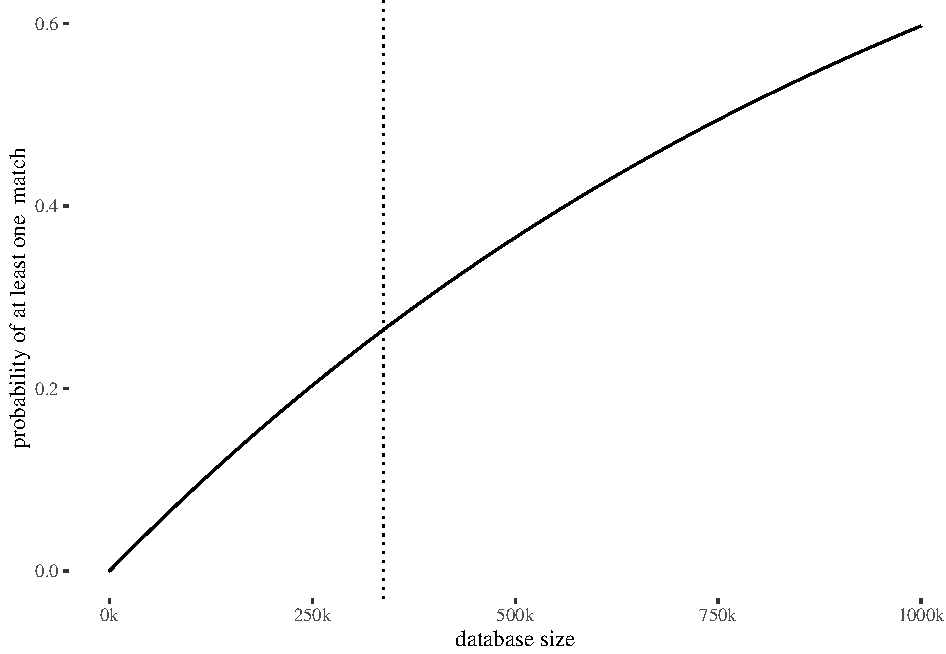
\includegraphics[width=0.8\linewidth]{lr-chapter_files/figure-latex/unnamed-chunk-4-1} 

}

\caption{Binomial model of the database search problem. The probability of at least one match depending on the database size, assuming independence and constant RMP used in  the Puckett case. The actual database size marked with a vertical line.}\label{fig:unnamed-chunk-4}
\end{figure}

If we use the RMP and database size used in the Puckett case, the
calculated probability of at least one match is 0.2645501. Not exactly
the DMP postulated by the defendant, but pretty close. The question is,
should this number be the probability used to evaluate the evidential
impact of the cold hit?

One problem is, the independence assumption is not satisfied in the
database search problem either (after all, since two arbitrary database
points very likely do not match, if you match one of them, you are much
less likely to match the other one). And the independence assumption is
not benign. We will illustrate it with a somewhat distand, but a very
striking example, coming from \todo{cite Barnett}. Suppose you consider
whether your effort of casting a vote in the upcoming election is worth
it in a context where there are 500k other voters. One of the
probabilities you might be interested in is the probability that your
vote would make a difference. If we apply the binomial model to the
problem, the probability that a candidate will receive exactly \(k\)
votes if \(n\) people vote is supposed to be
\({n \choose k} p^{k} (1-p)^{(n-k)}\), where votes of the population
members are supposed to be indepent and estimated to have the same
probability \(p\) of being for the candidate. For instance, if 500k
people vote and \(p= 0.5\), the probability that the candidate will
receive exactly 250k votes is 0.0011284, which is around
\nicefrac{1}{886} and much higher than \(\nicefrac{1}{n}\). This fairly
high chance made some claim that the chance that your voice is decisive
if the chances are equal is fairly high in such circumstances. However,
note that if \(p=.505\), the probability that the candidate will receive
exactly 250k votes is \ensuremath{1.5651281\times 10^{-14}}, which is
less than one in a trillion. This lead some
\todo{ Brennan and Lomasky, Democracy and
Decision, as well as Brennan, The Ethics of Voting, 19.} to claim that
outside of the very specific circumstances, decision-theoretic arguments
for the rationality of voting are hopeless. Barnett, \todo{Barnett}
however, points out that such a sensitivty to success probability simply
makes the binomial model inappropriate for the voting context, observing
that its calculations also disagree with empirical estimates which are
not too far from \(1/n\).
\todo{Andrew Gelman, Gary King, and W. John Boscardin, “Estimating the Probability of Events that Have Never Occurred: When Is Your Vote Decisive?” Journal of the American Statistical Association 93 (1998): 1–9; Gelman, Katz, and Tuerlinckx, “The Mathematics and Statistics of Voting Power”; and Casey Mulligan and
Charles Hunter, “The Empirical Frequency of a Pivotal Vote,” Public Choice 116 (2003):
31–54,} This sensitivity arises, because within the binomial model the
more trials (voters) there are, the more tightly the results will tend
to cluster around the probablity of success. To observe how unrealistic
that is, keep \(p=.505\) and ask yourself how probable it is that the
voting result will be between \(50.4\%\) and \(50.6\%\). Sure, this
outcome might be quite likely, but the binomial certainly overstimates
it at 0.8427212. Another unrealistic estimate obtained by the binomial
model is the estimate of the probability of an upset (that the leading
candidate will lose). With \(p=.505\) this is
\(\mathsf{pbinom(249999,500000,.505)}\), which turns out to be extremely
and unrealistically low: \ensuremath{7.5994495\times 10^{-13}}.

The bottom line of the above example is that if we have reasons to think
the independence assumption is not satisfied, the binomial model is not
appropriate. So, it seems, it is not appropriate for the database match
problem either. It is useful, in its simplicity, for illustrating an
important distinction whose conflation underlies one of the involved
arguments. YOu might have been surprised learning that while the expert
testified that RMP on 9 loci for Puckett was 1 in 1.1 million, Arizona
Department of Public Safety found 122 9-loci matches among 65,000
individuals. After all, 122/65000 is 0.0018769, which is much higher
than the reported RMP.

Probabilistic epistemology recommends that once we obtain new evidence,
our new degrees of belief should be the probabilities obtained by
conditionalizing on this evidence. Crucially, we should update on the
total evidence we obtained rather than only on a part of it. So here the
question is, does (General match hypothesis) exhaust what we have
learned from our database search?

To get us started thinking about this question, consider a coin analogy
which Donnelly \& Friedman (1999, p. 950) found more adequate than the
one proposed by the NRC. Imagine a biased coin whose physical appearance
is indistinguishable from the fair coins in a piggy bank. The biased
coin is the perpetrator and the piggy bank is the database containing
innocent people. After the biased coin is thrown into the bank with the
other coins, someone picks out a handful of coins at random and flips
each of them twenty times. Each coin lands heads approximately ten
times---except for one coin, which lands heads on all twenty flips. The
fact that other coins seem unbiased makes the claim that this one is
biased\\
better supported.

Coming back to DNA matches, think about the following scenario: first,
you identified the suspect by some means other than a database trawl.
Then, it turned out his DNA profile matches the crime scene stain. Fine,
here it seems uncontroversial that this constitutes strong further
incriminating evidence. Now, imagine a further database search for a
database not containing this suspect finds no matches. Would you think
that this information supports the guilt hypothesis? If your answer is
yes, then you do have the intuition that the lack of matches with other
people (whose profiles, in this particular case, happen to be in a
database) strengthens the evidence.

The key lesson here (and in the complete-world database scenario) is
that we not only learned that there was a match in the database, but
also that in \(d-1\) cases there was no match, and this information also
has evidential value.

Contrary to NRC II, \cite{donnelly1999DNADatabaseSearches} argue that if
potential suspects in the database are excluded as sources, this should
increase, not decrease, the probability that the defendant who matches
the crime traces is the source. A cold-hit match, then, is stronger and
not weaker evidence of guilty than ordinary DNA matches.

A detailed critical consideration of NRC II recommendation can be found
in (Donnelly \& Friedman, 1999).

However, the coin example involves

\%\paragraph{Shortcomings of the database match probability}

\%A database that contained everybody however, is \%a far-fetched
possibility. At least, the NRC II recommendation could very well apply
to more limited databases. Leaving coin tossing aside, another analogy
has been used to argue that the evidentiary value of a cold-hit match
should be weakened. The analogy is between searching for a match in a
database and multiple hypothesis testing, which is a dubious research
practice. In classical hypothesis testing, if the probability of type I
error in a single test of a hypothesis is 5\%, this probability will
increase by testing the same hypothesis multiple times. The database
match probability---the argument goes---would correct for the increased
risk of type I error. This analogy with multiple testing, however, is
misplaced. As \citet{balding2002DNDatabaseSearch} points out, multiple
testing consists in testing the \textit{same} hypothesis multiple times
against new evidence. In cold-hit cases, there is no such multiple
testing. \%there is no multiple hypothesis testing involved here.
\%Rather that the hypothesis about the suspect being formulated after
the test, Rather, multiple hypotheses---each concerning a different
individual in the database---are tested only once and then excluded if a
negative match occurs. \%before the search multiple individual
hypotheses about each of potential suspects in the database are
formulated, and each of them is tested once during the search. From this
perspective, the hypothesis that the defendant is the source was one of
the many hypotheses subject to testing. The cold-hit match supports that
hypothesis and rules out the others.

\paragraph{The likelihood ratio of cold-hit matches}

\%NRC II made another recommendation. They recommended that in cold-hit
cases the likelihood ratio \(R\) associated with the DNA match should be
divided by the size of the database \(d+1\). This recommendation, too,
is questionable. Suppose \(R\) is not too high, say because the
identified profile is common since the crime scene DNA is degraded and
only a few markers could be used. Then, \(d+1\) can be greater than
\(R\), so \(R/(d+1)<1\). The match would then be exculpatory, a very
counter-intuitive result. The recommendation seems mistaken on more
general grounds, as well. If the defendant on trial is the source, the
probability that he would match is practically 1. If he is not, the
probability that he would still match equals the random match
probability. Neither of these probabilities change because other
suspects have been tested in the database search. In fact, if potential
suspects are excluded as potential sources,this should increases, not
decrease, the probability that the defendant who matches the crime
traces is the source.

A more principled way to assess cold-hit matches, one based on the
likelihood ratio, exists. The proposal draws from the literature on the
so-called \emph{island problem}, studied by
\citet{eggleston1978evidence}, \citet{dawid1994island}, and
\citet{dawid1996CoherentAnalysisForensic}. Let the prosecutor's
hypothesis \(H_p\) be
\texttt{The\ suspect\ is\ the\ source\ of\ the\ crime\ traces\textquotesingle{}\ and\ the\ defense\textquotesingle{}s\ hypothesis\ \$H\_d\$\ be}The
suspect is not the source of the crime traces'. Let \(E\) be the DNA
match between the crime stain and the suspect (included in the database)
and \(D\) the information that no one among the \(N-1\) profiles in the
database matches the crime stain. The likelihood ratio associated with
\(E\) and \(D\) should be
\citep{balding1996EvaluatingDNAProfilea, taroni2006bayesian}: \%

\begin{align*}
V & = \frac{\pr(E,D\vert H_p)}{\pr(E,D\vert H_d)}.
\end{align*}

\% Since \(\pr(A\wedge B)=\pr(A\vert B)\pr(B)\), for any statement \(A\)
and \(B\), this ratio can be written as \%

\begin{align*}
V & = \frac{\pr(E\vert H_p,D)}{\pr(E\vert H_d,D)} \times \frac{\pr(D\vert H_p)}{\pr(D\vert H_d)}.
\end{align*}

\% The first ratio \(\nicefrac{\pr(E\vert H_p,D)}{\pr(E\vert H_d,D)}\)
is roughly \(\nicefrac{1}{\gamma}\), where \(\gamma\) is the random
match probability. The second ratio
\(\nicefrac{\pr(D\vert H_p)}{\pr(D\vert H_d)}\)--- call it the
\emph{database search ratio}---requires some more work. Consider first
the denominator \(\pr(D \vert H_d)\). If the suspect is not the source
(\(H_d\)), someone else is, either someone who is in the database or
someone not in the database. Let \(S\) stand for `The source is someone
in the database.' By the law of total probability, \%

\begin{align*}
\pr(D\vert H_d) & = \pr(D\vert S, H_d) \pr(S\vert H_d) + \pr(D\vert \neg S, H_d) \pr(\neg S \vert H_d). 
\end{align*}

\% If the source is someone in the database (\(S\)) and the suspect is
not the source (\(H_d\)), it is very unlikely that no one in the
database would match (\(D\)). \%the probability of \(D\) that no one
other than the suspect would match can be set to zero. So
\(\pr(D\vert S, H_d)\approx 0\). \%The above equality therefore
simplifies to \%

\begin{align*}
\pr(D\vert H_d) & =  \pr(D\vert \neg S, H_d) \pr(\neg S %\vert H_d), 
\end{align*}

The database search ratio would therefore be: \%

\begin{align*}
\frac{\pr(D\vert H_p)}{\pr(D\vert H_d)} & = \frac{\pr(D\vert H_p)}{\pr(D\vert \neg S, H_d) \pr(\neg S \vert H_d)}.
\end{align*}

\% Note that \(\pr(D\vert H_p)=\pr(D\vert \neg S, H_d)\) because whether
the suspect is the source (\(H_p\)) or not (\(H_d\)) does not affect
whether there is a match in a database that does not contain the source
(\(\neg S\)).\% \%and let ---the probability that no person in the
database other than the suspect would match (D), assuming the suspect
was in fact the source---be \(\psi_{N-1}\). \%Notice that
\(\pr(D\vert \neg S, H_d)\) \% is the probability that no one other than
the suspect matches in the database that does not contain the real
source, if the suspect is not the source. But , so this conditional
probability can also be estimated as \(\psi_{N-1}\).
\footnote{If the prior probability that the perpetrator is in the database was high, the calculations would need to be different. But normally, this prior isn't too high.}
Let \(\pr(S | H_d)=\varphi\). The database search ratio then would
reduce to \%

\begin{align*}
\frac{\pr(D\vert H_p)}{\pr(D\vert H_d)} & = \frac{1}{1-\varphi}.
\end{align*}

\% As the database gets larger, \(\varphi\) increases and the database
search ratio also increases. This ratio equals one only if no one in the
database could be the source, that is, \(\varphi=0\).

Since the likelihood ratio \(V\) of the cold-hit match results by
multiplying the likelihood ratio of the DNA match and the database
search ratio, \(V\) will always be greater than the mere likelihood
ratio of the match (except for the unrealistic case in which
\(\varphi=0\)) . Thus, a cold-hit DNA match should count as stronger
evidence than a DNA match of a previously identified suspect.
\citet{dawid1996CoherentAnalysisForensic} study different database
search strategies and consider the possibility that information about
the match is itself uncertain, but the general point remains. Under
reasonable assumptions, ignoring the database search would give a
conservative assessment of the evidentiary strength of the cold-hit
match.\footnote{\citet{donnelly1999DNADatabaseSearches}, with slightly different assumptions, derived the formula $R \times [1+mD/N]$, where $R = 1/\gamma$, $D$ is the database size, $N$ the number of people in population not in database, and $m$ is an optional multiplier reflecting how much more likely persons in the database are though to be the source when compared to the rest of the population. The expression cannot be less than $\gamma$. If no other profile has been tested, $D=0$ and LR is simply the regular DNA match LR. If $N$ is zero, that is, everyone in population is in the database, the result is infinitely large.}

This proposal is able to accommodate different competing intuitions.
First, consider the intuition that as the size of the database grows, it
is more likely that someone in the database would match. This intuition
is captured by the fact that \(\varphi\) increases proportionally to the
size of the database even though this increase does not imply that the
evidential value of the cold-hit match should decrease. Second, there is
intuitive resistance in basing a conviction on a cold-hit match,
although this resistance is less strong in case of an ordinary match
(more on this later in Section \ref{sec:naked}). This preference for
convictions based on an ordinary DNA match seems in tension with the
claim that a cold-hit match is stronger evidence of guilt than an
ordinary match. There is a way to reconcile both sides, however. The key
is to keep in mind that the evidentiary strength---measured by the
likelihood ratio---should not be confused with the posterior probability
of guilt given the evidence. \%Even if a cold-hit match is stronger
evidence of guilty, this fact does not imply that the posterior
probability of the defendant's guilt should be higher. If the cold-hit
match is the only evidence of guilt, the posterior probability of guilt
may well be lower compared to cases in which other evidence, such as
investigative leads, supplements the DNA match. This lower posterior
probability would justify the intuitive resistance towards convictions
in cold-hit cases despite the stronger probative value of cold-hit
matches in themselves.

\%What about the intuition that we'd be uneasy about a conviction based
solely on a cold hit match, much less than about a DNA-match based
conviction of a previously and independently identified suspect? We
think so because now we're thinking about the posterior probability
given total evidence.

As the preceding discussion shows, the likelihood ratio is a fruitful
conceptual framework for assessing the strength of the evidence, even in
complex cases such as cold-hits. One major difficulty, however, is the
choice of the hypotheses \(H\) and \(H'\) that should be compared.
Generally speaking, the hypotheses should in some sense compete with one
another---say, in a criminal trial, \(H\) is the hypothesis put forward
by the prosecution and \(H'\) is the hypothesis put forward by the
defense. \%\todo{slightly modified the last sentence} Presumably, the
two hypotheses should be something that the two parties disagree about.
But this minimal constraint offers too little guidance and leaves open
the possibility for manipulations and misinterpretations of the
evidence. What follows outlines some of the main arguments in the
literature on this topic.

\paragraph{Ad hoc hypotheses and Barry George}

Consider a stylized DNA evidence case. Suppose the prosecutor puts
forward the hypothesis that the suspect left the traces found at the
crime scene. This hypothesis is well supported by laboratory analyses
showing that the defendant genetically matches the traces. The defense,
however, responds by putting forward the following \textit{ad hoc}
hypothesis: `The crime stain was left by some unknown person who
happened to have the same genotype as the suspect.' Since the
probability of the DNA match given either hypothesis is 1, the
likelihood ratio equals 1 \citep{evett2000MoreHierarchyPropositions}.
The problem generalizes. For any item of evidence and any given
prosecutor's hypothesis \(H\), there is an \textit{ad hoc} competing
hypothesis \(H^*\) such that
\(\nicefrac{\pr(E \vert H)}{\pr(E \vert H^*)}=1\). Hypothesis \(H^*\) is
a just-so hypothesis, one that is selected only because it explains the
evidence just as well as hypothesis \(H\) does \citep{mayo2018}. \% If
no further constraints are placed on the choice of the competing
hypotheses---it would seem---no evidence could ever incriminate a
defendant. This is unsettling. \%But this conclusion need not be so
damning in practice. Judges and jurors, however, will often recognize
\textit{ad hoc} hypotheses for what they are---artificial theories that
should not be taken seriously. Perhaps, the reasonable expectations of
the participants in a trial will suffice to constrain the choice of
hypotheses in just the right way. At the same time, real cases can be
quite complex, and it is not always obvious whether a certain choice of
competing hypotheses, which are not obviously \textit{ad hoc}, is
legitimate or not.

\%\paragraph{Barry George}

\%Even when the competing hypotheses are not obviously \textit{ad hoc},
\%the absence of a clear rationale for their choice \%may create
confusions in the assessment of the evidence.

A notable example is R.~v.~Barry George (2007 EWCA Crim 2722). Barry
George was accused of murdering TV celebrity Jill Dando. \%
\%\textbackslash{}begin\{center\}
\%\textbackslash{}begin\{tabular\}\{lp\{12cm\}\} \% \(E\) \&\\
A single particle of firearm residue \%(FDR) was found one year later in
George's coat pocket and it matched the residue from the crime scene.
This was the key incriminating evidence against him.
\%\textbackslash{}end\{tabular\} \%\textbackslash{}end\{center\} \%
\%\noindent  The defense argued that, since it was only one particle,
there must have been contamination. The experts for the prosecution,
however, testified that it was not unusual that a single particle would
be found on the person who fired the gun. George was convicted, and his
first appeal was unsuccessful. \% After the first appeal, Dr.~Evett from
the Forensic Science Service worried that the evidence had not been
properly assessed at trial. The jurors were presented with the
conditional probability \%\(\pr(\textsf{residue}\vert H_d)\) of finding
the firearm residue in George's coat given the defense hypothesis
\%\(H_d\) that George \textit{did not} fire the gun. This probability
was estimated to be quite low, indicating that the evidence spoke
against the defense's hypothesis. But the jurors were not presented with
the conditional probability \%\(\pr(\textsf{residue}\vert H_p)\) of
finding the same evidence given the prosecutor's hypothesis \%\(H_p\)
that George \textit{did} fire the gun that shot Dando. \%
\%\textbackslash{}begin\{center\} \%
\textbackslash{}begin\{tabular\}\{lp\{12cm\}\} \%\(H_d\) \& BG did not
fire the gun that shot JD.\textbackslash{} \%\(H_p\) \& BG fired the gun
that shot JD. \%\textbackslash{}end\{tabular\}
\%\textbackslash{}end\{center\} \% \noindent  An expert witness,
Mr.~Keeley, was asked to provide both conditional probabilities and
estimated them to be \(\nicefrac{1}{100}\), which indicated that the
firearm residue had no probative value. \%After new guidelines for
reporting low level FDR in 2006, the FSS re-assessed the evidence and
concluded that it was irrelevant. George appealed again in 2007, and
relying on Keely's estimates, won the appeal. \%

At first, this case seems a good illustration of how likelihood ratios
help to correctly asses the value of the evidence presented at trial.
But this reading of the case would be overly optimistic. In fact, a
close study of the trial transcript shows that Keeley's choice of
hypotheses lacked coherence and the likelihood ratio based on them was
therefore meaningless \citep{fenton2014WhenNeutralEvidence}. \% \% For
instance, Mr Keeley is reported to have said: \%
\%\textbackslash{}begin\{quote\} \% It was necessary to balance the
likelihood that the particle came from a gun fired by the appellant and
the likelihood that it came from some other source. Both were unlikely
but both were possible. \%\textbackslash{}end\{quote\} \%\noindent  \%
On one occasion, Keeley compared the hypothesis that the particle found
in George's pocket came from a gun fired by George himself, and the
alternative hypothesis that the particle came from another source. \%At
the same time, Keeley said that the prior probabilities of both
hypotheses should be low, which is mathematically impossible if they
were exhaustive and exclusive.\\
On another occasion, Keeley took the prosecutor's hypothesis to be
\texttt{The\ particle\ found\ in\ George\textquotesingle{}s\ pocket\ came\ from\ the\ gun\ that\ killed\ Dando\textquotesingle{}.\ \ But\ the\ \ conditional\ probability\ of\ the\ evidence\ given\ this\ hypothesis\ should\ not\ be\ low.\ It\ should\ actually\ be\ one.\ \ \%\textbackslash{}dots\ \%\textbackslash{}begin\{quote\}\ \%\textbackslash{}dots\ \ Mr\ Keeley\ gave\ to\ us,\ this\ was\ an\ equally\ unlikely\ event,\ whether\ it\ had\ come\ from\ the\ cartridge\ that\ killed\ Miss\ Dando,\ or\ from\ some\ innocent\ source.\ \ \%\textbackslash{}end\{quote\}\ \%\ \%\textbackslash{}noindent\ Note\ that\ here\ the\ persecution\ hypothesis\ is\ taken\ to\ be:\ \textbackslash{}emph\{the\ particle\ found\ in\ BG\textquotesingle{}s\ pocket\ came\ from\ the\ gun\ that\ killed\ JD\}.\ Now,\ \$E\$\ is\ a\ logical\ consequence\ of\ this\ hypothesis,\ and\ so\ this\ likelihood\ should\ be\ 1.\ \ \ In\ some\ other\ contexts,\ Keeley\ took\ the\ defense\ hypothesis\ to\ be}The
particle on George's pocket was inserted by contamination', but again,
the conditional probability of the evidence given this hypothesis should
be one. The most charitable reading of the trial transcript suggests
that the expert had in mind the hypotheses
\texttt{George\ was\ the\ man\ who\ shot\ Dando\textquotesingle{}\ and}The
integrity of George's coat was corrupted'. But \%these hypotheses are
neither exhaustive nor exclusive, and Keeley gave no clear criterion for
why these hypotheses should be compared in the likelihood ratio
\citep[see][for further details]{fenton2014WhenNeutralEvidence}.

\paragraph{Exclusive and exhaustive?}

The confusion in the Barry George case is attributable to the absence of
clear rules for choosing the hypotheses in the likelihood ratio. One
such rule could be: pick competing hypotheses that are exclusive (they
cannot be both true) and exhaustive (they cannot be both false). In this
way, the parties would not be able to pick \textit{ad hoc} hypotheses
and skew the assessment of the evidence in their own favor. \% \%One of
the competing hypotheses in the likelihood ratio does not have to be the
negation of the other. In some cases, they could both be false (hence,
not exhaustive), and in some they could both be true (hence, not
mutually exclusive).\\
\% Besides blocking partisan interpretations of the evidence, there are
other principled reasons to follow the exclusive-and-exhaustive rule,
specifically, the fact that when the hypotheses are not exclusive or
exhaustive, the likelihood ratio delivers counterintuitive results.
\%andconfusions in the assessment of the strength of the evidence often
arise. \% \%but it is not obvious that the hypotheses selected should
always be exclusive and exhaustive. \%Whether this rule would be a good
guiding principle, however, is not clear-cut. \%

If two competing hypotheses \%\(H_p\) and \(H_d\) are not mutually
exclusive, it is possible that \%the evidence supports them to an equal
extent \%\todo{This was wrong. Fixed.} they both make the evidence
equally likely (the likelihood ratio is one), and yet the posterior
probabilities of the hypotheses given the evidence are higher than their
prior probabilities. For instance, let \(H_p\) stand for
\texttt{The\ defendant\ is\ guilty\textquotesingle{}\ and\ \$H\_d\$\ for}The
defendant was not at the crime scene'. Both hypotheses might be true.
\%Say the prior probability of both is \(50\%\). Let \(E\) stand for
\texttt{Ten\ minutes\ before\ the\ crime\ took\ place\ the\ defendant-\/-\/-seen\ at\ a\ different\ location-\/-\/-\ was\ overheard\ on\ the\ phone\ saying\ \textbackslash{}emph\{go\ ahead\ and\ kill\ him\}.\textquotesingle{}\ \ \%\$E\$\ supports\ both\ \$H\_p\$\ and\ \$H\_d\$,\ and\ \ It\ is\ conceivable\ that\ the\ likelihood\ ratio\ should\ equal\ one\ in\ this\ context,\ yet\ the\ posterior\ probabilities\ of\ each\ hypothesis,\ given\ \$E\$,\ should\ be\ higher\ than\ the\ prior\ probability.\ So,\ intuitively,\ the\ evidence\ should\ positively\ support\ each\ hypothesis,\ contrary\ to\ what\ the\ likelihood\ ratio\ would\ suggest.\ \ \%\ Further,\ when\ the\ two\ competing\ hypotheses\ are\ not\ exhaustive,\ the\ likelihood\ ratio\ may\ once\ again\ clash\ with\ our\ intuitions.\ \ \%The\ likelihood\ ratio\ might\ then\ equal\ one\ even\ though\ the\ evidence\ lowers\ their\ posterior\ probability.\ \ For\ example,\ suppose\ Fred\ and\ Bill\ attempted\ to\ rob\ a\ man.\ The\ victim\ resisted,\ was\ struck\ on\ the\ head\ and\ died.\ Say\ \$H\_p\$\ stand\ for}Fred
struck the fatal blow' and \(H_d\) stand for
\texttt{Bill\ struck\ the\ fatal\ blow.\textquotesingle{}\ The\ hypotheses\ are\ not\ exhaustive.\ A\ missing\ hypothesis\ is}The
man did not die from the blow.' Suppose \(E\) is the information that
the victim had a heart attack six months earlier. The likelihood ratio
\(\nicefrac{\pr(E \vert H_p)}{\pr(E \vert H_d)}\) equals one since
\(\pr(E\vert H_p)=\pr(E\vert H_d)\). Yet \(E\) reduces the probability
of both \(H_p\) and \(H_d\). So, in this case, the evidence should
negatively support each hypothesis, contrary to what the likelihood
ratio suggests.

Despite these problems, however, always relying on exclusive and
exhaustive hypotheses is not without complications either. For consider
an expert who decides to formulate the defense hypothesis by negating
the prosecution hypothesis, say,
\texttt{the\ defendant\ did\ not\ hit\ the\ victim\ in\ the\ head.\textquotesingle{}\ This\ choice\ of\ defense\ hypothesis\ can\ be\ unhelpful\ in\ assessing\ the\ evidence\ because\ the\ required\ probabilities\ are\ hard\ to\ estimate.\ For\ instance,\ what\ is\ the\ probability\ that\ the\ suspect\ would\ carry\ such\ and\ such\ blood\ stain\ if\ he\ did\ not\ hit\ the\ victim\ in\ the\ head?\ This\ depends\ on\ whether\ he\ was\ present\ at\ the\ scene,\ what\ he\ was\ doing\ at\ the\ time\ and\ many\ other\ circumstances.\ \%Similarly,\ in\ a\ rape\ case,\ it\ is\ hard\ to\ estimate\ the\ probability\ of\ the\ matching\ evidence\ if\ the\ suspect\ did\ not\ have\ the\ intercourse\ with\ the\ victim.\ Instead,\ what\ is\ considered\ is\ the\ hypothesis\ that\ someone\ else,\ unrelated\ to\ the\ suspect,\ had\ intercourse\ with\ the\ victim.\ \ As\ \textbackslash{}citet\{evett2000MoreHierarchyPropositions\}\ point\ out,\ the\ choice\ of\ a\ particular\ hypothesis\ to\ be\ used\ in\ the\ evaluation\ of\ the\ strength\ of\ the\ evidence\ \ \%of,\ say,\ the\ lack\ of\ semen\ in\ a\ rape\ case,\ \ \ will\ depend\ on\ contextual\ factors.\ \%Sometimes\ it\ will\ be\ \textbackslash{}emph\{intercourse\ did\ not\ take\ place\},\ sometimes\ it\ will\ be\ \textbackslash{}emph\{the\ intercourse\ took\ place,\ but\ the\ complainant\ used\ a\ vagina\ douche\},\ or\ sometimes\ \textbackslash{}emph\{another\ sexual\ act\ took\ place\}.\ \ More\ often\ than\ not,\ the\ hypotheses\ chosen\ will\ not\ be\ mutually\ exclusive.\ \ \%\ Comparing\ exclusive\ and\ exhaustive\ hypotheses\ can\ also\ be\ unhelpful\ for\ jurors\ or\ judges\ making\ a\ decision\ at\ trial.\ \ \%is\ not\ required\ for\ the\ application\ of\ Bayes\textquotesingle{}\ Theorem,\ is\ not\ the\ usual\ practice,\ and\ could\ lead\ to\ a\ \ In\ a\ paternity\ case,\ for\ example,\ \%\ in\ which\ the\ results\ of\ DNA\ profiling\ \ are\ to\ be\ evaluated,\ \ the\ expert\ should\ not\ compare\ the\ hypotheses}The
accused is the father of the child' and its negation, but rather,
\texttt{The\ accused\ is\ the\ father\ of\ the\ child\textquotesingle{}\ and}The
father of the child is a man unrelated to the putative father'
\citep{biedermann2014UseLikelihoodRatio}. The choice of the latter pair
of competing hypotheses is preferable. Even though the relatives of the
accused are potential fathers, considering such a far-fetched
possibility would make the assessment of the evidence more difficult
than needed \%Similarly, for a given DNA mixture, strictly speaking for
any \(n\) there is a hypothesis that covers the suspect and \(n\) other
unkown sources, but for sufficiently large \(n\) these are usually
discarded as unrealistic. \% \%At the same time, if the defense
hypothesis is too specific, \textit{ad hoc} and entails the evidence, it
won't be of much use. For example, take
\texttt{The\ crime\ stain\ was\ left\ by\ some\ unknown\ person\ who\ happened\ to\ have\ the\ same\ genotype\ as\ the\ suspect.\textquotesingle{}\ \%The\ probability\ of\ a\ DNA\ match\ given\ this\ hypothesis\ would\ be\ 1.\ \ \%But\ usually\ the\ probability\ of\ the\ DNA\ match\ given\ the\ prosecution\textquotesingle{}s\ hypothesis,\ say}The
crime stain was left by the suspect,' is also 1. This would result in a
rather uninformative likelihood ratio of 1 \%For example, consider the
prosecution hypothesis The probability of a match given this hypothesis
is practically 1.\% Another feature of such specific explanations is
that it's hard to reasonably estimate their prior probability, and so
hard to use them in arguments between opposing sides.
\citep{evett2000MoreHierarchyPropositions}.

\paragraph{Variability}

Any choice of competing hypotheses lies between two extremes. For one
thing, exclusive and exhaustive hypotheses guard against arbitrary
comparisons and ensure a more objective assessment of the evidence. The
drawback is that exhaustive and exclusive hypothesis cover the entire
space of possibilities, and sifting through this space is cognitively
unfeasible. So, in this respect, comparing more circumscribed hypotheses
is preferable. The danger of doing so, however, is slipping into
arbitrariness as likelihood ratios heavily depend on the hypotheses that
are compared. The more latitude in the choice of the hypotheses, the
more variable the likelihood ratio as a measure of evidentiary value.
\%It is hard not to view this variability as a sign of arbitrariness.
\%\% R; this last sentence was too much

Here is a particularly troubling \%example phenomenon.
\%\todo{changed, because this wasn't really an example.} Competing
hypotheses can concern any factual dispute, from minute details such as
whether the cloth used to suffocate the victim was red or blue, to
ultimate questions such as whether the defendant stabbed the victim.\\
As it turns out, the likelihood ratio varies across hypotheses
formulated at different levels of granularity: offense, activity and
source level hypotheses (on this distinction, see earlier in
\ref{subsec:levels}). It is even possible that, at the source level, the
likelihood ratio favors one side, say the prosecution, but at the
offence level, the likelihood ratio favors the other side, say the
defense, even though the hypotheses at the two levels are quite similar.
Further, a likelihood ratio that equals 1 when source level hypotheses
are compared may tip in favor of one side or the other when offence
level hypotheses are compared \citep{fenton2014WhenNeutralEvidence}.
This variability makes the likelihood ratio a seemingly arbitrary---and
easily manipulable---measure of evidentiary value. This is not to say
that it is unhelpful. Expert witnesses often rely on the likelihood
ratio when they assess the probative value of many forms of evidence
\citep{enfs2015}.\\
\% The likelihood ratio can be misleading, but this risk is mitigated
when its assessment is accompanied by a careful discussion of a number
of issues, such as: which hypotheses are being compared; how they are
formulated; their level of granularity (that is, source, activity and
offense level); why the hypotheses are (or are not) exclusive and
exhaustive; why other hypotheses are ruled out as unworthy of
consideration.

\%the choice of the hypotheses to be compared, their level, their being
exclusive and exhaustive (or not), the formulation of the evidential
statement, and the reasons not to use other hypotheses in the evidence
evaluation.

\%\todo{Revised this paragraph a bit, take a look again.} \%M: Great,
nice summary. I changed a few things here and there

\% \%

\%It is unclear, however, how the analogy translates to cold-hit cases.
Searching a larger database no doubt increases the probability of
finding a match at some point. But judges and jurors should not be
concerned with \%the probability of the statement \%The NRC II
recommendation pertained to the probability of the statement
\%\texttt{At\ least\ one\ of\ the\ profiles\ in\ the\ database\ \%of\ size\ \$d\$\ would\ randomly\ match\ the\ crime\ sample.\textquotesingle{}\ \%Call\ it\ the\ general\ match\ hypothesis.\ \ \%This\ statement\ has\ probability\ \$(d+1)\textbackslash{}times\ p\$,\ where\ \$p\$\ is\ the\ random\ match\ probability\ and\ \$d+1\$\ is\ the\ database\ size.\ \ \textbackslash{}todo\{Is\ this\ right?\ You\ have\ d+1.\ Why?\}\ \%\ \ \%are\ interested\ in\ whether\ a\ particular\ defendant\ is\ the\ source\ of\ the\ crime\ traces.\ \%They\ are\ concerned\ with\ the\ statement}The
profile of the particular defendant on trial would randomly match the
crime sample.`Call this the particular match hypothesis. \%and the
probability of at least one false positive. \%So what is of interest is
the probability of the particular, not the general match hypothesis. \%
This is in line with the general idea that one should update on total
available evidence: the claim that the defendant's profile match entails
but is not entailed by the claim that at least one of the database
profiles match, and so it is the former and not the latter that the
fact-finders should rely on. \% \%Rather, they should be concerned with
\%the probability of the statement `The profile of the defendant on
trial would randomly match the crime sample.' The probability of finding
a match between the particular defendant and the crime sample does not
increase because other people in the database are tested. \%

\%NRC II was concerned with the fact that in cold-hit cases the
identification of a particular defendant occurs after testing several
individuals. This concern has to do with the data-dependency of one's
hypothesis. But, as \citet{balding2002DNDatabaseSearch} points out, the
problem of data-dependency arises when the same hypothesis is tested
multiple times against new evidence. In cold-hit cases, however, there
is no multiple testing. \%there is no multiple hypothesis testing
involved here. \%Rather that the hypothesis about the suspect being
formulated after the test, \%Rather, multiple hypotheses---each
concerning a different individual in the database---are tested only once
and are excluded by a negative match. \%before the search multiple
individual hypotheses about each of potential suspects in the database
are formulated, and each of them is tested once during the search.
\%From this perspective, the hypothesis that the defendant is the source
was one of the many hypotheses subject to testing. The cold-hit match
supports that hypothesis and rules out the others.

\%Perhaps, there is a better analogy here
\%\citep[p.\ 950]{donnelly1999DNADatabaseSearches}. Imagine a coin that
is known to be biased but whose physical appearance makes it
indistinguishable from the fair coins in a piggy bank. The biased coin
is the perpetrator and the \%piggy bank is the database containing
innocent people. \%After the biased coin is thrown into the bank with
the other coins, someone picks out a handful of coins at random and
flips each of them twenty times. Each coin lands heads approximately ten
times---except for one coin, which lands heads on all twenty flips. The
fact that other coins seem unbiased makes the claim that this one is
biased better supported since at least one coin in the bank must be
biased.\%

\% \%Contrary to NRC II, \cite{donnelly1999DNADatabaseSearches} argue
that if potential suspects in the database are excluded as sources, this
should increase, not decrease, the probability that the defendant who
matches the crime traces is the source. A cold-hit match, then, is
stronger and not weaker evidence of guilty than ordinary DNA matches.

\% \%This can be made clear by relying on the likelihood ratio as a
measure of the evidential strength of the cold-hit DNA match. If the
defendant on trial is the source, the probability that he would match is
practically 1. If he is not, the probability that he would still match
equals the random match probability. Neither of these probabilities
change because other suspects have been tested in the database search.
In fact, if potential suspects are excluded as potential sources, \%this
should increases, not decrease, the probability that the defendant who
matches the crime traces is the
source.\footnote{Of course, a classical statistician might refuse to rely on Bayesian reasoning, and rely on classical hypothesis testing instead. There are various good reasons not to do so, but we'll just point out that in such a case they simply have nothing to say about the posterior probability of the identity claim.}
\% \%Since the focus should not be on the particular, not the general
match hypothesis, the coin tossing analogy does not work. \%In a DNA
trawl you're not repeating an experiment to reject a general hypothesis.
Rather, you consider a particular hypothesis
(\emph{the defendant is the source of the material}) and test once for
\emph{the defendant's profile matches the crime sample}, and once for
each claim of type
\emph{person $i$ in the database does not have a matching profile}.

\%moved this bit to a footnote

\%NRC II made another recommendation. They recommended that in cold-hit
cases the likelihood ratio \(R\) associated with the DNA match should be
divided by \(d+1\). Their first recommendation was about a correction of
the random match probability (that is, to multiply it by the size of the
database), and this second recommendation is about the likelihood ratio
(that is, to divide it by \(d+1\)). This has counterintuitive
consequences. Suppose \(R\) is not too high, say because the identified
profile is common since the crime scene DNA is degraded and only a few
markers could be used. Then, \(d+1\) can be greater than \(R\), so
\(R/(d+1)<1\). The match would be exculpatory, a very counter-intuitive
result.

\%Moreover, NRC II would entail that if the police pick a random person
from the database, test their profile and it is a match (call this
\emph{lucky strike} )and don't test other members of the database, this
evidence --- if we follow NRC II --- should be stronger than a unique
hit in a systematic database trawl, which also does not seem too
convincing. \% \%Interestingly, the frequentist argument focused on a
different hypothesis than the likelihood one. The former assessed the
probability that at least one profile in the database would match the
crime sample by chance, the latter focused on the hypothesis that
exactly one profile would match. \%In the case of frequency,
multiplication by \(D+1\) results in a conservative and imprecise
estimate, while in the case of likelihood, division by \(D+1\) is
supposed to give a precise calculation of the likelihood of a cold hit.
\%

\% \%emphasized that, in cold-hit cases, the likelihood ratio should
taken into account that the suspect is identified only after the search
not before. If this fact is not taken into account the likelihood ratio
would be data dependent. \% \%who argued that the hypotheses proposed by
the critics of NRC II are data dependent, because the suspect is
identified only after the search (see Subsection \ref{subse:LRlogical}
for further details). \%

\%Commented this out, perhaps, this is not needed

\%(3 CT 669, 675; 5 CT 1093.)11

\% How do we square the supposedly extremely low DNA profile frequency
with the seemingly high match frequency in empirical studies on existing
databases? The key difference is between the probability of a particular
previously selected profile matching one in the database, and the
probability of the database containing \emph{some} match. \%
{[}MARCELLO'S COMMENTS: YES, YOU MADE THIS POINT EARLIER WHEN YOU
CRITICIZED THE USE OF DMP, SO I DON'T THINK THIS SHOULD BE REPEATED
HERE. MAYBE YOU CAN JUST CLARIFY WHAT YOU SAID EARLIER WHEN YOU
DISTINGUISHED DMP FROM RMP?{]}

\% Continuing with the die example, say I pick number one as my
\texttt{suspect,\textquotesingle{}\textquotesingle{}\ and\ my\ database\ has\ \$n=5\$\ with\ individual}profile
frequency in the population'' of \(\nicefrac{1}{6}\). On the assumption
that the database is randomly drawn from the population (with
replacement), the probability of one of the numbers in the database
being 1 is \(\approx 1-0.6=0.4\) (notice this time the database can
contain repetitions and the sampling was random and so we can't use
addition to calculate \(\pr(\textrm{no match with 1})\)). \%
{[}MARCELLO'S COMMENT: I REALLY LOST YOU HERE. NOW YOU SEEM TO BE
ADDRESSING A DIFFERENT PROBLEM THAN COLD-HIT MATCHES. {]}

\% In contrast, there are \(6^5\) possible states of the database, and
\(6\times 5 \times 4\times 3 \times 2\) of them contain no repetitions,
so \(\pr(\textrm{no match})\) is \(\approx 0.093\) and the probability
of \emph{a} matching pair being present in the database is
\(\approx 0.91\). Intuitively, the difference arises because now we're
searching through \({ 5 \choose 2}=10\) different pairs looking for any
of the 6 possible profile matches, instead of searching through 5
profiles looking exactly for one
profile.\footnote{This is  a reformulation of the well-known birthday problem, it's just we discussed it using smaller numbers to make the considerations more intuitively compelling.}
\% {[}MARCELLO'S COMMENTS: OK, SO HERE YOU SEEM TO BE ADDRESSING ANOTHER
PROBLEM, SUCH AS BIRTHDAY PROBLEM AND RELATED. I WONDER IF THIS IS
ANOTHER PROBLEM, NOT IMMEDIATELY HAVING TO DO WITH COLD-HIT DNA MATCHES.
CAN THIS GO INTO A SEPARATE SUBSECTION? THAT MIGHT HELP ORIENT THE
READER AND NOT MAKE THIS ONE SUBSECTION SO LONG.{]}

\%\subsection{Sensitivity of LR to hypothesis choice and NRC II} \label{subsec:LRandDNA}

\%This approach has also been defended defended by
\%\citet{stockmarr1999LikelihoodRatiosEvaluating} who points out that
since the suspect is identified after the databases search, the
hypothesis is formulated \textit{ad hoc}. Without the correction, then,
the likelihood ratio would be data-dependent.

\%Recalling the discussion of sensitivity of the likelihood ratio to the
choice of hypotheses, let's take a look at an interesting attempt to
defend NRC II by \citet{stockmarr1999LikelihoodRatiosEvaluating}. He
insists that hypotheses such as
\emph{JS was one of the crime scene donors} are evidence-dependent in
the case of database search, ``since we had no way of knowing prior to
the search that Smith would be the person that matched'' (p.~672).
Instead, Stockmarr insists, we should evaluate LR using hypotheses that
can be formulated prior to the search, such as
\emph{the true perpetrator is among the suspects identified from the database}.
And indeed, the likelihood of this hypothesis is as NRC II suggests,
\(\nicefrac{k}{np}\), where \(k\) is the number of matching profiles,
\(n\) the database size, and \(p\) the random match probability
\citep[see][for a derivation]{stockmarr1999LikelihoodRatiosEvaluating}.

\%Dawid, in a discussion with Stockmarr
\citep{dawid2001CommentStockmarrLikelihood} points out that Stockmarr's
hypotheses, while not depending on the result of the search, depend on
the data themselves (because they change with the database size). More
importantly, he also indicates that Stockmarr's hypotheses are composite
and the assessment of LR therefore requires additional assumptions about
the priors. Once these are used with Stocmarr's own LR, the posterior is
the same as the one obtained using the methods proposed by the critics
of NCR II. The phenomenon is a particular case of the one we already
discussed, because Stockmarr's hypothesis and the one originally used in
the database search problem are equivalent conditional on the evidence.
This turns out to be another example of how LR on its own might be
insufficiently informative, especially when it is unclear what the
involved hypotheses
are.\footnote{See however, Stockmarr's own reply (\emph{ibidem}).}

\%\subsection{Resolving the Database Search Problem}

\%So we know not to use DMP. But the question remains: what's the
relation between the value of a DNA match in a cold hit case as compared
to a DNA match for a previously and independently identified suspect?
After all we need to have a justified stance on cold hit evidence, and
there seems to be no hope of reaching one without the tools provided by
legal probabilism.

\%Various versions of probabilistic calculations have been developed,
depending on what idealizations and additional complexities are being
considered. \%In order to better understand how to properly assess a
cold-hit match, it is instructive to consider a simple scenario, the
\emph{island problem}, studied by \citet{eggleston1978evidence},
\citet{dawid1994island}, and
\citet{dawid1996CoherentAnalysisForensic}.\todo{M: Nowhere do you talk about the island problem. Did you delete something here?}

\%\%Let \(H_p\) stand for
\texttt{The\ suspect\ is\ the\ source\ of\ the\ crime\ traces\textquotesingle{}\ and\ \$H\_d\$\ for}The
suspect is not the source of the crime traces'. Let evidence \(E\) be
the DNA match between the crime stain and the suspect (included in the
database) and \(D\) the information that no one among the \(N-1\)
profiles in the database matches the crime stain. The likelihood ratio
associated with \(E\) and \(D\) should be
\citep{balding1996EvaluatingDNAProfilea, taroni2006bayesian}: \%

\begin{align*}
V & = \frac{\pr(E,D\vert H_p)}{\pr(E,D\vert H_d)}
\end{align*}

\% \%Since \(\pr(A\wedge B)=\pr(A\vert B)\pr(B)\), for any statement
\(A\) and \(B\), this ratio can be written as \%

\begin{align*}
V & = \frac{\pr(E,\vert H_p,D)}{\pr(E\vert H_d,D)} \times \frac{\pr(D\vert H_p)}{\pr(D\vert H_d)}
\end{align*}

\% \%The ratio \(\nicefrac{\pr(E,\vert H_p,D)}{\pr(E\vert H_d,D)}\) is
roughly \(\nicefrac{1}{\gamma}\), where \(\gamma\) is the random match
probability. The ratio \(\nicefrac{\pr(D\vert H_p)}{\pr(D\vert H_d)}\)
is called the \emph{database search ratio}. To determine this ratio,
consider first the denominator \(\pr(D \vert H_d)\). If the suspect is
not the source, someone else is, either someone who is in the database
or someone not in the database. Let \(S\) stand for `The source is
someone in the database.' By the law of total probability, \%

\begin{align*}
\pr(D\vert H_d) & = \pr(D\vert S, H_d) \pr(S\vert H_d) + \pr(D\vert \neg S, %H_d) \pr(\neg S \vert H_d)  
\end{align*}

\% \%Note that if the source is someone in the database (\(S\)) and the
suspect is not the source (\(H_d\)), it is nearly impossible that no one
in the database would match (\(D\)). \%the probability of \(D\) that no
one other than the suspect would match can be set to zero.
\%\todo{Is this right? I elaborated what you had. Please check!} So
\(\pr(D\vert S, H_d)\approx 0\). The above equation \%therefore
simplifies to: \%

\begin{align*}
\pr(D\vert H_d) & =  \pr(D\vert \neg S, H_d) \pr(\neg S \vert H_d)  
\end{align*}

\% \%Let \(\pr(D\vert H_p)\) \%be \(\psi_{N-1}\). \%Notice that
\(\pr(D\vert \neg S, H_d)\) \%is the probability of a random match in a
database of size \(N-1\) not containing the the real source, and can
also be estimated as \(\psi_{N-1}\).
\todo{I don't follow the reasoning. Can you clarify? Why do these two probabilities equal the same thing?}
If \(\pr(S)=\varphi\), then the second ratio in our calculation of \(V\)
therefore reduces to: \%

\begin{align*}
\frac{\psi_{N-1}}{\psi_{N-1}(1-\varphi)} & = \frac{1}{1-\varphi}
\end{align*}

\% \%As the database gets larger, \(\varphi\) increases and the database
search ratio also increases. This ratio equals one only if no one in the
database could be the source, that is, \(\varphi=0\).

\%Since in order to obtain the likelihood ratio \(V\), the likelihood
ratio of the DNA match is multiplied by the database search ratio, the
result will alwaysbe greater than the mere likelihood ratio of the match
(except for the unrealistic case in which \(\varphi=0\)) . Thus, a
cold-hit DNA match should count as stronger evidence than a DNA match of
a previously identified suspect.
\citet{dawid1996CoherentAnalysisForensic} study variations of the
database search problem, with different search strategies and including
the possibility that information about the match is itself uncertain,
but the general point remains. Under reasonable assumptions, ignoring
the search errs on the side of
caution.\footnote{\citet{donnelly1999DNADatabaseSearches}, with slightly different assumptions, derived the formula $R \times [1+mD/N]$, where $R = 1/\gamma$, $D$ is the database size, $N$ the number of people in population not in database, and $m$ is an optional multiplier reflecting how much more likely persons in the database are though to be the source when compared to the rest of the population. The expression cannot be less than $\gamma$. If no other profile has been tested, $D=0$ and LR is simply the regular DNA match LR. If $N$ is zero, that is, everyone in population is in the database, the result is infinitely large. }

\%Think about the following scenario: first, you identified the suspect
by some means. Then, it turned out his DNA profile matches the crime
scene stain. Fine. Now, imagine further database search for a database
not containing this suspect finds no matches. Would you think that this
information supports the guilt hypothesis? If your answer is yes, then
you do have the intuition that the lack of matches with other people
(whose profiles, in this particular case, happen to be in a database)
strengthens the evidence.

\%The fact that, compared to an ordinary DNA match, a cold-hit DNA match
is stronger evidence of guilty does not imply that the posterior
probability of the defendant's guilt should be higher in cold-hit cases.
The other evidence used to first identify the suspect, jointly with the
DNA match, might result in a higher posterior probability of guilt, even
if the likelihood ratio of the cold-hit match is higher. This different
in the posterior probability of guilt accounts for the intuition that in
cold-hit cases we should resist conviction so long as the evidence only
consists of a DNA match. The resistance toward conviction should be less
strong in other cases so long as the DNA match is supplemented by other
incriminating evidence.

\%What about the intuition that we'd be uneasy about a conviction based
solely on a cold hit match, much less than about a DNA-match based
conviction of a previously and independently identified suspect? We
think so because now we're thinking about the posterior probability
given total evidence.

\subsection{Levels of Hypotheses}\label{levels-of-hypotheses}

\todo{Consider using the stuff that was  commented out! I left percentage signs.}

Difficulties in assessing probabilities go hand in hand with the choice
of the hypotheses of interest. To some approximation, hypotheses can be
divided into three levels: offence, activity, and source level
hypotheses. At the offence level, the issue is one of guilt or
innocence, as in the statement
\texttt{Smith\ intentionally\ attacked\ the\ victim\ with\ a\ knife\textquotesingle{}.\ \ At\ the\ activity\ level,\ hypotheses\ \ do\ not\ include\ information\ about\ intent\ but\ simply\ describe\ what\ happened\ and\ what\ those\ involved\ did\ or\ did\ not\ do.\ An\ example\ of\ activity\ level\ hypothesis\ is}Smith
bled at the scene.`Finally, source level hypotheses describe the source
of the traces, such as `Smith left the stains at the crime scene,'
without specifying how the traces got there. Overlooking differences in
hypothesis level can lead to serious confusions.

To illustrate, consider a case in which a DNA match is the primary
incriminating evidence. In testifying about the DNA match at trial,
experts will often assess the probability that a random person,
unrelated to the crime, would coincidentally match the crime stain
profile \%For a survey of developments and complications of this model,
see \citep{foreman2003interpreting}. The random match probability is
often an impressively low number, say 1 in 100 million or lower, at
least excluding the possibility that relatives or identical twins would
coincidentally match
\citep{donnelly1995NonindependenceMatchesDifferent}.

\%This low probability indicates that it is extremely unlikely that a
random person would match.

\%The match should count as strong evidence against the defendant \% See
\%This presentation is similar to classical hypothesis testing. In such
a context one starts by setting up a chance hypothesis, often called the
null \(H_0\), and then calculates the probability of the evidence (or
data obtained) being such as it is or more extreme on the assumption
that \(H_0\) holds. If this probability is small (conventionally, below
\(0.01\) or \(0.05\)), this counts as evidence against \%\(H_0\). But
note that just because \(\pr(E\vert H_0)\) is small, it does not follow
that, for any alternative hypothesis, \(H_*\) \(\pr(E\vert H_*)\) is
large. The latter probability could be equally low.\\
\% \%A DNA profile consists of pairs of alleles at several loci.
Individual allele probabilities are used to calculate the expected
frequency of a given profile \(\Gamma\) in a relevant population, so
that we obtain the genotype probability \(\gamma\). Assuming the
so-called Hardy-Weinberg equilibrium, \(\gamma\) can be obtained by
multiplying the allele probabilities. Very roughly, the probability of a
match at any particular locus is around \(\nicefrac{1}{10}\), and so the
probability of a match on all 20 loci used by the FBI CODIS system
should be \(\left(\nicefrac{1}{10}\right)^{20}\). \% \%Such
calculations, however, are a bit simplistic. One factor is that given
the crime stain, we already know that at least one population member has
profile \(\Gamma\), and the observation of a gene increases the chance
of another of the same type. Actual calculations are quite complicated,
\citep[see][]{taroni2006bayesian}, as we'll discuss in the section on
BNs for DNA evidence evaluation. \% \%In legal context, \(\gamma\) ---
the so-called Random Match Probability (RMP), that is, the probability
that a random person from the population matches the crime stain profile
--- is taken to be the probability that the suspect is a match if in
fact he is innocent and is usually estimated as the frequency of a given
profile in the relevant population. \% \% is not the probability of
innocence (see \ref{sec:fallacies} for details), it \% \%And yet, in
what way the match counts as evidence against the \%defendant is not
straightforward. \%Here it is paramount to avoid a number of confusions.
\% \% \%First, the random match probability is not the posterior
probability of innocence since
\(\pr(\textsf{match} \vert \textsf{innocence})\) should not be confused
with \(\pr(\textsf{innocence} \vert \textsf{match})\). \%The random
match probability speaks to the former, not the latter probability. \%To
confuse the two would be to commit the prosecutor's fallacy (see
\ref{sec:fallacies} for details). \%Second, \%Since the random match
probability low probability indicates that it is extremely unlikely that
a random person would match. It is tempting to equate the random match
probability to \(\pr(\textsf{match} \vert \textsf{innocence})\) and
together with the prior \(\pr(\textsf{innocence})\) use Bayes' theorem
to calculate\\
the posterior probability of innocence
\(\pr(\textsf{innocence} \vert \textsf{match})\). But this would be a
mistake. \% Applying Bayes' theorem is of course recommended and helps
to avoid the prosecutor's fallacy, the conflation of
\(\pr(\textsf{innocence} \vert \textsf{match})\) and
\(\pr(\textsf{match} \vert \textsf{innocence})\). \%(see
\ref{sec:fallacies} for details). The problem lies elsewhere. Equating
the random match probability with
\(\pr(\textsf{match} \vert \textsf{innocence})\) overlooks the
difference between offense, activity and source level hypothesis. It is
hasty to assume that, in one way or another, a DNA match can speak
directly to the question of guilt or innocence. Even if the suspect
actually left the genetic material at the scene---source level
proposition---the match does not establish guilt. \%The match could be
the result of a laboratory error. Or Even if the defendant did visit the
scene and came into contact with the victim, it does not follow that he
committed the crime he was accused of. \%So even if the random match
probability is usually very low, it does not follow that the posterior
probability of innocence is near the random match probability given by
the expert. \%It is true, however, that in many circumstances the random
match probability and the posterior probability of innocence given a
match would both be very low.

Few forms of evidence can speak directly to offense level hypotheses.
Circumstantial evidence that is more amenable to a probabilistic
quantification, such as DNA matches and other trace evidence, does not.
Eyewitness testimony may speak more directly to offense level
hypotheses, but it is also less easily amenable to a probabilistic
quantification. This makes it difficult to assign probabilities to
offense level hypotheses. Experts are usually not supposed to comment
directly on offense level hypotheses, but they often comment on activity
level and source level hypotheses. In moving from source to activity
level, however, additional sources of uncertainty come into play.
\%\citep{Cook1998hierarchy}. \% The assessment of activity level
hypotheses depends on additional variables other than those on which the
assessment of source level hypotheses depends. \%For example, is this
the kind of staining that would occur if the suspect kicked the victim
in the head? For example, the probability of finding such and such
quantity of matching glass if the suspect smashed the window depends on
how the window was smashed, when it was smashed, and what the suspect
did after the action. Another problem arises due to recent improvements
in DNA profiling technology \citep{Cook1998hierarchy}. Since today
investigators are able to obtain profiles from minimal amounts of
genetic material, transfer probabilities become more difficult to assess
as more opportunities of transfer arise. If small traces such as dust
speckles can be used as evidence, the possibility that the traces were
brought to the scene accidentally becomes more likely. For this reason,
moving beyond source level hypotheses requires a close collaboration
between scientists, investigators and attorneys
\citep[see][for a discussion]{Cook1998hierarchy}. \%The hypotheses
themselves are up for revision as evidence is obtained or facts about
what happened are accepted \citep{evett2000MoreHierarchyPropositions}.

\% \% \% \%Since the likelihood ratio might change with the choice of
the hypotheses, the clarity on the choice of the hypotheses, and their
level in particular, is crucial. For instance, \% \% \%

\subsection{The two-stain problem}\label{the-two-stain-problem}

\todo{Also, worth a discussion as an illustration}

A case study that further illustrates both advatanges and limitations of
the likelihood ratio as a measure of evidentiary strength is the
two-stain problem, originally formulated by \cite{Evett1987}. The key
limitation is due to the combination of two circumstances: first, that
likelihood ratios vary depending on the choice of hypotheses being
compared; second, that it is not always clear which hypotheses should be
compared. To illustrate what is at stake, what follows begins with
Evett's original version of the two-stain problem (which does not pose
any challenge to the likelihood ratio) and then turns to a more complex
version (which suggests that likelihood ratios, in and of themselves,
are insufficiently informative).

\paragraph{Evett's two-stain problem}

Suppose two stains from two different sources were left at the crime
scene, and the suspect's blood matches one of them. More precisely, the
two items of evidence are as follows: \%

\begin{center}
    \begin{tabular}{lp{12cm}} 
        $E_1$ & The blood stains at the crime scene are of types $\gamma_1$ and $\gamma_2$ of estimated  frequencies $q_1$ and $q_2$ respectively.\\
        $E_2$ & The suspect's blood type is $\gamma_1$. 
    \end{tabular}
 \end{center}

\% Let the first hypothesis be that the suspect was one of the two men
who committed the crime and the second hypothesis the negation of the
first. \%

\begin{center}
    \begin{tabular}{lp{12cm}} 
        $H_p$ & The suspect was one of the two men who committed the crime.\\
        $H_d$ & The suspect was not one of the two men who committed the crime.
    \end{tabular}
 \end{center}

\% \cite{Evett1987} shows that the likelihood ratio of the match
relative to these two hypotheses is \(\nicefrac{1}{2q_1}\) where \(q_1\)
is the estimated frequency of the characteristics of the first stain.
Surprisingly, the likelihood ratio does not depend on the frequency
associated with the second stain.

To understand Evett's argument, consider first the likelihood ratio:

\begin{align*}
\frac{\pr(E_1\wedge E_2\vert H_p)}{
    \pr(E_1\wedge E_2\vert H_d)} & = \frac{\pr(E_1 \vert E_2 \wedge H_p)}{
    \pr(E_1 \vert E_2 \wedge H_d)
    }\times 
 \frac{\pr(E_2\vert H_p)}{\pr(E_2 \vert H_d)}. 
 \end{align*}

\noindent Notice that the suspect's blood type as reported in \(E_2\) is
independent of whether or not he participated in the crime, that is,
\(\pr(E_2\vert H_p)=\pr(E_2 \vert H_d)\). So the likelihood reduces to:

\begin{align*}
 \frac{\pr(E_1\wedge E_2\vert H_p)}{
    \pr(E_1\wedge E_2\vert H_d)} & = \frac{\pr(E_1 \vert E_2 \wedge H_p)}{
    \pr(E_1 \vert E_2 \wedge H_d).
 } \end{align*}

\noindent
 The numerator \(\pr(E_1 \vert E_2 \wedge H_p)\) is the probability that
one of the stains is \(\gamma_1\) and the other \(\gamma_2\) given that
the suspect is guilty and has profile \(\gamma_1\). The probability that
one of the stains is \(\gamma_1\) is simply 1, and assuming blood type
does not affect someone's propensity to commit a crime, the probability
that the second stain is \(\gamma_2\) equals its relative frequency in
the population, \(q_2\). So the numerator is \(1\times q_2 = q_2\). \%
Next, consider the denominator \(\pr(E_1 \vert E_2 \wedge H_d)\). If
\(H_d\) is true, \%the fact that the suspect has profile \(\gamma_1\) is
irrelevant for the crime scene profiles. the crime was committed by two
randomly selected men with profiles \(\gamma_1\) and \(\gamma_2\). \%who
can be seen as two random samples from the general population as far as
their blood profiles are concerned. There are two ways of picking two
men with such profiles (\(\gamma_1,\gamma_2\) and
\(\gamma_2,\gamma_1\)), each having probability \(q_1q_2\). So the
denominator equals \(2q_1q\). By putting numerator and denominator
together, \%

\begin{align*}
 \frac{q_2}{2q_1q_2} = \frac{1}{2q_1}. 
 \end{align*}

\% \noindent which completes the argument. In general, if there are
\(n\) bloodstains of different phenotypes, the likelihood ratio is
\(\nicefrac{1}{nq_1}\), or in other words, the likelihood ratio depends
on the number of stains but not on the frequency of the other
characteristics.

\paragraph{A more complex two-stain problem}

Consider now a more complex two-stain scenario. Suppose a crime was
committed by two people, who left two stains at the crime scene: one on
a pillow and another on a sheet. John Smith, who was arrested for a
different reason, genetically matches the DNA on the pillow, but not the
one on the sheet. What likelihood ratio should we assign to the DNA
match in question? \cite{meester2004WhyEffectPriora} argue that there
are three plausible pairs of hypotheses associated with numerically
different likelihood ratios (see their paper for the derivations). The
three options are listed below, where \(R\) is the random match
probability of Smith's genetic profile and \(\delta\) the prior
probability that Smith was one of the crime scene donors. \%

\begin{center}
    \footnotesize
    \begin{tabular}{@{}p{5cm}p{5cm}l@{}}
        \toprule
        $H_p$ & $H_d$  & LR \\ \midrule
        Smith was one of the crime scene donors.   &  Smith was not one of the crime scene donors. & $\nicefrac{R}{2}$   \\
        Smith was the pillow stain donor.     & Smith was not one of the crime scene donors.& $R$\\
        Smith was the pillow stain donor. & Smith was not the pillow stain donor. &  $\nicefrac{R(2-\delta)}{2(1-\delta)}$
        \\ \bottomrule
    \end{tabular}
\end{center}

\normalsize

\noindent

Two facts are worth noting here. First, even though the likelihood
ratios associated with the hypotheses in the table above are numerically
different, the hypotheses are in fact equivalent conditional on the
evidence. After all, Smith was one of the crime scene donors just in
case he was the pillow stain donor, because he is excluded as the stain
sheet donor. Smith was not one of the crime scene donors just in case he
was not the pillow stain donor, because he is excluded as the sheet
stain donor.\\
\% \%Second, the example illustrates that sometimes the likelihood ratio
is sensitive to the prior probability (after all, \(\delta\) occurs in
the third likelihood ratio in the table). \% In addition, even though
the likelihood ratios are numerically different, their posterior
probabilities given the evidence are the same. To see why, note that the
prior odds of the three \(H_p\)'s in the table should be written in
terms of \(\delta\). Following \cite{meester2004WhyEffectPriora}, the
prior odds of the first hypothesis in the table are
\(\nicefrac{\delta}{1-\delta}\). The prior odds of the second hypothesis
are \(\nicefrac{(\delta/2)}{(1-\delta)}\). The prior odds of the third
hypothesis are \(\nicefrac{(\delta/2)}{(1-(\delta/2))}\). In each case,
the posterior odds --- the result of multiplying the prior odds by the
likelihood ratio --- are the same:
\(R\times \nicefrac{\delta}{2(1-\delta)}\). So despite differences in
the likelihood ratio, the posterior odds of equivalent hypotheses are
the same so long as the priors are appropriately related (this point
holds generally).

\citet{dawid2004likelihood} cautions that the equivalence of hypotheses,
conditional on the evidence, does not imply that they can all be
presented in court. He argues that the only natural hypothesis for the
two-stain problem is that Smith is guilty as charged.
\cite{meester2004ResponseDawidBalding} reply that focusing on the guilt
hypothesis is beyond the competence of expert witnesses who should
rather select pairs of hypotheses on which they are competent to
comment. Some such pairs of hypotheses, however, will not be exclusive
and exhaustive. When this happens, as seen earlier, the selection of
hypotheses is prone to arbitrariness. To avoid this problem,
\cite{meester2004WhyEffectPriora} recommend that the likelihood ratio
should be accompanied by a tabular account of how a choice of prior odds
(or prior probabilities) will impact the posterior odds, for a sensible
range of priors (for a general discussion of this strategy called
sensitivity analysis, see earlier discussion in \ref{subsec:sensi-ana}).
In this way, the impact of the likelihood ratio is made clear, no matter
the hypotheses chosen. This strategy concedes that likelihood ratios, in
and of themselves, are insufficiently informative, and that they should
be combined with other information, such as a range of priors, to allow
for an adequate assessment of the
evidence.\footnote{The reference class problem 
is lurking in the background.  \citet{balding2004comment} argues that, in order to calculate the probability of a match given the evidence, the class of possible culprits should be identified, and  different choices of such a class might lead to different likelihood ratios. On the problem of priors, see \ref{subsec:prior}. On the reference class problem, see \ref{sec:reference}.}

\% and prior odds needed to calculate LR in cases in which LR depends on
priors are available. \% \%\textbackslash{}footnote\{Further discussion
of the phenomenon is quite interesting. \%

\paragraph{Likelihood ratio variability in cold-hit cases}

\%The sensitivity of the likelihood ratio to the choice of hypotheses is
not confined to the two-stain problem or alike scenarios.

A similar conclusion holds for DNA matches in cold-hit cases. When the
suspect is identified through a database search of different profiles,
\cite{taroni2006bayesian} and \cite{balding1996EvaluatingDNAProfilea}
have argued that the likelihood ratio of the match \%---which usually
equals 1/\(\gamma\) where \(\gamma\) is the random match probability---
should be adjusted by the database search ratio (see earlier in
\ref{subsec:cold-hit} for details). This proposal tacitly assumes that
the hypothesis of interest is something like
\texttt{the\ defendant\ is\ the\ true\ source\ of\ the\ crime\ traces.\textquotesingle{}\ \%This\ assumption\ is\ eminently\ plausible\ but\ not\ uncontroversial.\ \ \ \%The\ National\ Research\ Council\ \ (NRC\ II)\ recommended\ in\ 1996\ that\ that\ the\ likelihood\ ratio\ of\ the\ match\ 1/\$\textbackslash{}gamma\$\ be\ divided\ by\ the\ size\ of\ the\ database.\ In\ defending\ this\ proposal,\ \ In\ contrast,\ \textbackslash{}cite\{stockmarr1999LikelihoodRatiosEvaluating\},\ who\ defends\ the\ NRC\ II\ 1996\ \ recommendation,\ argues\ \ that\ the\ likelihood\ ratio\ of\ the\ match\ in\ cold-hit\ cases\ should\ be\ divided\ by\ the\ size\ of\ the\ database.\ He\ points\ out\ that\ the\ hypothesis}the
defendant is the true source of the crime traces' is evidence-dependent
because the investigators had no way of knowing prior to the search that
anyone in particular would match. \% (p.~672). Accordingly, Stockmarr
believes we should evaluate the likelihood ratio using hypotheses that
can be formulated prior to the database search, such as `The true source
of the crime traces is among the suspects in the database.' The
likelihood associated with this hypothesis and its negation is
\(\nicefrac{k}{np}\), where \(k\) is the number of matching profiles,
\(n\) the database size, and \(p\) the random match probability
\citep[see][for a derivation]{stockmarr1999LikelihoodRatiosEvaluating}.

In response to this argument, Dawid points out that even though
Stockmarr's hypothesis does not depend on the result of the search, it
still depends on the data themselves (because it changes with the
database size) \citep{dawid2001CommentStockmarrLikelihood}. Dawid also
points out that Stockmarr's hypothesis is composite and thus the
assessment of the likelihood ratio requires additional assumptions about
the priors. Once these assumptions are made clear, the posterior of
Stockmarr's hypothesis is the same as that of other hypotheses.
\%obtained using others methods.\\
This phenomenon is a particular case of what we discussed earlier since
the hypothesis `The true source is among the suspects in the database'
(Stockmarr's) and the hypothesis `The defendant is the true source of
the crime traces' (Taroni's) are equivalent conditional on the evidence.
\%\todo{I changed this is a bit. Is this correct?}
\%\todo{Yes, there was a minor confusing one passage before, fixed.}
This is another example of how likelihood ratios on their own might be
insufficiently informative to allow for an adequate assessment of the
evidence.

\subsection{LR \& relevance, small-town murder
etc.}\label{lr-relevance-small-town-murder-etc.}

The U.S.~Federal Rules of Evidence define relevant evidence as one that
has `any tendency to make the existence of any fact that is of
consequence to the determination of the action more probable or less
probable than it would be without the evidence' (rule 401). This
definition is formulated in a probabilistic language. Legal probabilists
interpret it by relying on the likelihood ratio, a standard
probabilistic measure of evidential relevance
\citep{lempert1977modeling,lyon1996relevance,aitken2004statistics, aitken2010fundamentals,sullivan2016LikelihoodStoryTheory}.
The likelihood ratio (initially introduced in \ref{sec:odd-bayes} and
more extensively in Section \ref{sec:LR}) is the probability of
observing the evidence given that the prosecutor's or plaintiff's
hypothesis is true, divided by the probability of observing the same
evidence given that the defense's hypothesis is true.

Let \(E\) be the evidence, \(H\) the prosecutor's or plaintiff's
hypothesis, and \(H'\) the defense's hypothesis. The likelihood ratio
\%\(LR(E, H, H')\) is defined as follows: \%

\begin{align*}LR(E,H,H') & = \frac{P(E\vert H)}{P(E\vert H')}\end{align*}

\% On this interpretation, relevance depends on the choice of the
competing hypotheses. \%\(H_p\) and \(H_d\) are used as examples, but
other competing hypotheses \(H\) and \(H'\) could also be used. \%When
there are no ambiguities, \(LR(E, H_p, H_d)\) will be shortened into the
less cumbersome \(LR(E)\). \% A piece of evidence is relevant---in
relation to a pair of hypotheses \(H\) and \(H'\)---provided the
likelihood ratio \(LR(E, H, H')\) is different from one and irrelevant
otherwise. For example, the bloody knife found in the suspect's home is
relevant evidence in favor of the prosecutor's hypothesis because we
think it is far more likely to find such evidence if the suspect
committed the crime (prosecutor's hypothesis) than if he didn't
(defense's hypothesis) \%\citep[7]{finkelstein2009basic}
\citep{finkelstein2009basic}. In general, for values greater than one,
\(LR(E, H, H')>1\), the evidence supports the prosecutor's or
plaintiff's hypothesis \(H\), and for values below one,
\(LR(E, H, H')<1\), the evidence supports the defense's hypothesis
\(H'\). If the evidence is equally likely under either hypothesis,
\(LR(E, H, H')=1\), the evidence is considered irrelevant.

\subsection{The Small Town Murder objection}

This account of relevance has been challenged by cases in which the
evidence is intuitively relevant and yet its likelihood ratio, arguably,
equals one. Here is one of them: \%One such case is
\emph{Small Town Murder}

\begin{quote}
    \emph{Small Town Murder:} A person accused of murder in a small town was seen driving to the small town at a time prior to the murder. The prosecution's theory is that he was driving there to commit the murder. The defense theory is an alibi: he was driving to the town because his mother lives there to visit her. The probability of this evidence if he is guilty equals that if he is innocent, and thus the likelihood ratio is 1 \dots %, and under what is suggested as the ``Bayesian'' analysis, it is therefore irrelevant. 
    Yet, every judge in every trial courtroom of the country would admit it [as relevant evidence]. %, and I think everyone on this list would say it is relevant. 
    %And so we have a puzzle.  
    \citep[The difficulty has been formulated by Ronald Allen, see the discussion in][]{park2010BayesWarsRedivivus}
    \end{quote}

\noindent  Counterexamples of this sort abound. Suppose a prisoner and
two guards had an altercation because the prisoner refused to return a
food tray. The prisoner had not received a package sent to him by his
family and kept the tray in protest. According to the defense, the
prisoner was attacked by the guards, but according to the prosecution,
he attacked the guards. The information about the package sent to the
prisoner and the withholding of the tray fails to favor either version
of the facts, yet it is relevant evidence
\citep{pardo2013NaturePurposeEvidence}. \%Counterexamples of this sort
abound.

\begin{itemize}
\item In response to an eyewitness testimony the defendant claims that his identical twin is the culprit. The testimony is unable to favor any of the two options and yet is considered relevant. 
\item  Suppose the evidence at issue is that a fight occurred and the only dispute is over who started it. 
\item  Or suppose the defendant was stopped because of speeding  three minutes after an aborted bank robbery and $\nicefrac{1}{2}$ a mile away from the site. The prosecution says this is evidence of guilt: it shows the defendant was escaping. The defense responds that this is evidence of innocence: no bank robber would speed and attract attention. 
\item Or, in a murder case, the defendant is the victim's son. Is that relevant to show he’s guilty? Is it relevant to show he's innocent? The answer seems to be yes, to both questions. 
This example is due to Samuel Gross 
and is discussed in \citep{park2010BayesWarsRedivivus}. 
\end{itemize}

\%In general, there seem to be numerous examples in which evidence is,
intuitively relevant, and the evidence supports neither side's theory
over the other side's theory. How is such evidence to be judged relevant
from the probabilist perspective?

\%\subsection{Replies to the overlapping evidence objection}

\%In response (inspired by the ideas put forward in the discussion by
David Kaye, Bruce Hay and Roger Park), note that

It is true that if a piece of evidence \(E\) fits equally well with two
competing hypotheses \(H\) and \(H'\), then \(P(E\vert H)=P(E\vert H')\)
and thus \(LR(E,H,H')\) will equal 1. But the likelihood ratio may
change depending on the selection of hypotheses. Rule 401 makes clear
that relevant evidence should have `any tendency to make the existence
of \emph{any fact that is of consequence} {[}emphasis ours{]} to the
determination of the action more probable or less probable'. So the
range of hypotheses to compare should be quite broad. Just because the
likelihood ratio equals one for a specific selection of \(H\) and
\(H'\), it does not follows that it equals one for \textit{any}
selection of \(H\) and \(H'\) which are of consequence to the
determination of what happened. In \textit{Small Town Murder}, whether
the suspect was in town at all is surely of consequence for determining
what happened (if he was not in town, he could not have committed the
crime). The fact that he was seen driving is helpful information for
establishing whether or not he was in town.

But if the range of hypotheses \(H\) and \(H'\) to compare in the
likelihood ratio \(LR(E, H, H')\) is quite broad, this may raise another
concern. The choice of hypotheses needed to determine the relevance of
an item of evidence might depend on other items of evidence, and so it
might be difficult to determine relevance until one has heard all the
evidence. This fact --- Ronald Allen and Samuel Gross argue in
\citep{park2010BayesWarsRedivivus} --- makes the probabilistic account
of relevance impractical. But, in response, David Kaye points out that
deciding whether a reasonable juror would find evidence \(E\) helpful
requires only looking at what hypotheses or stories the juror would
reasonably consider. Since the juror will rely on several clues about
which stories are reasonable, this task is computationally easier than
going over all possible combinations of hypotheses
\citep{park2010BayesWarsRedivivus}.

\%\subsection{Small Town Murder and bayesian networks}\label{sec:smalltownBN}

Legal probabilists can also offer a more principled response to
\emph{Small Town Murder} and related problems based on Bayesian
networks. \%rather than a reasonable choice of the competing hypotheses.
\%The emphasis on the logical relations between the hypotheses have been
used by Fenton to address the . Let \(H_p\) be the prosecutor's
hypothesis that the defendant committed the murder, and \(H_d\) the
defense's hypothesis that the defendant was visiting his mother. Let
\(E\) be the fact that the defendant was seen driving to the town prior
to the murder. Further, suppose the prior probabilities of \(H_d\) and
\(H_p\) are \(50\%\), and the conditional probability of \(E\) on each
of those hypotheses is \(70\%\) (nothing of what will be said depends on
this particular choice of values). Crucially, while indeed the evidence
supports both hypotheses, this example is based on a pair of hypotheses
that are neither mutually exclusive nor exhaustive. A Bayesian network
can be used to calculate other likelihood ratios for hypotheses that are
exclusive and exhaustive.

\%

\begin{figure}[!h]
    \begin{floatrow}
        \ffigbox{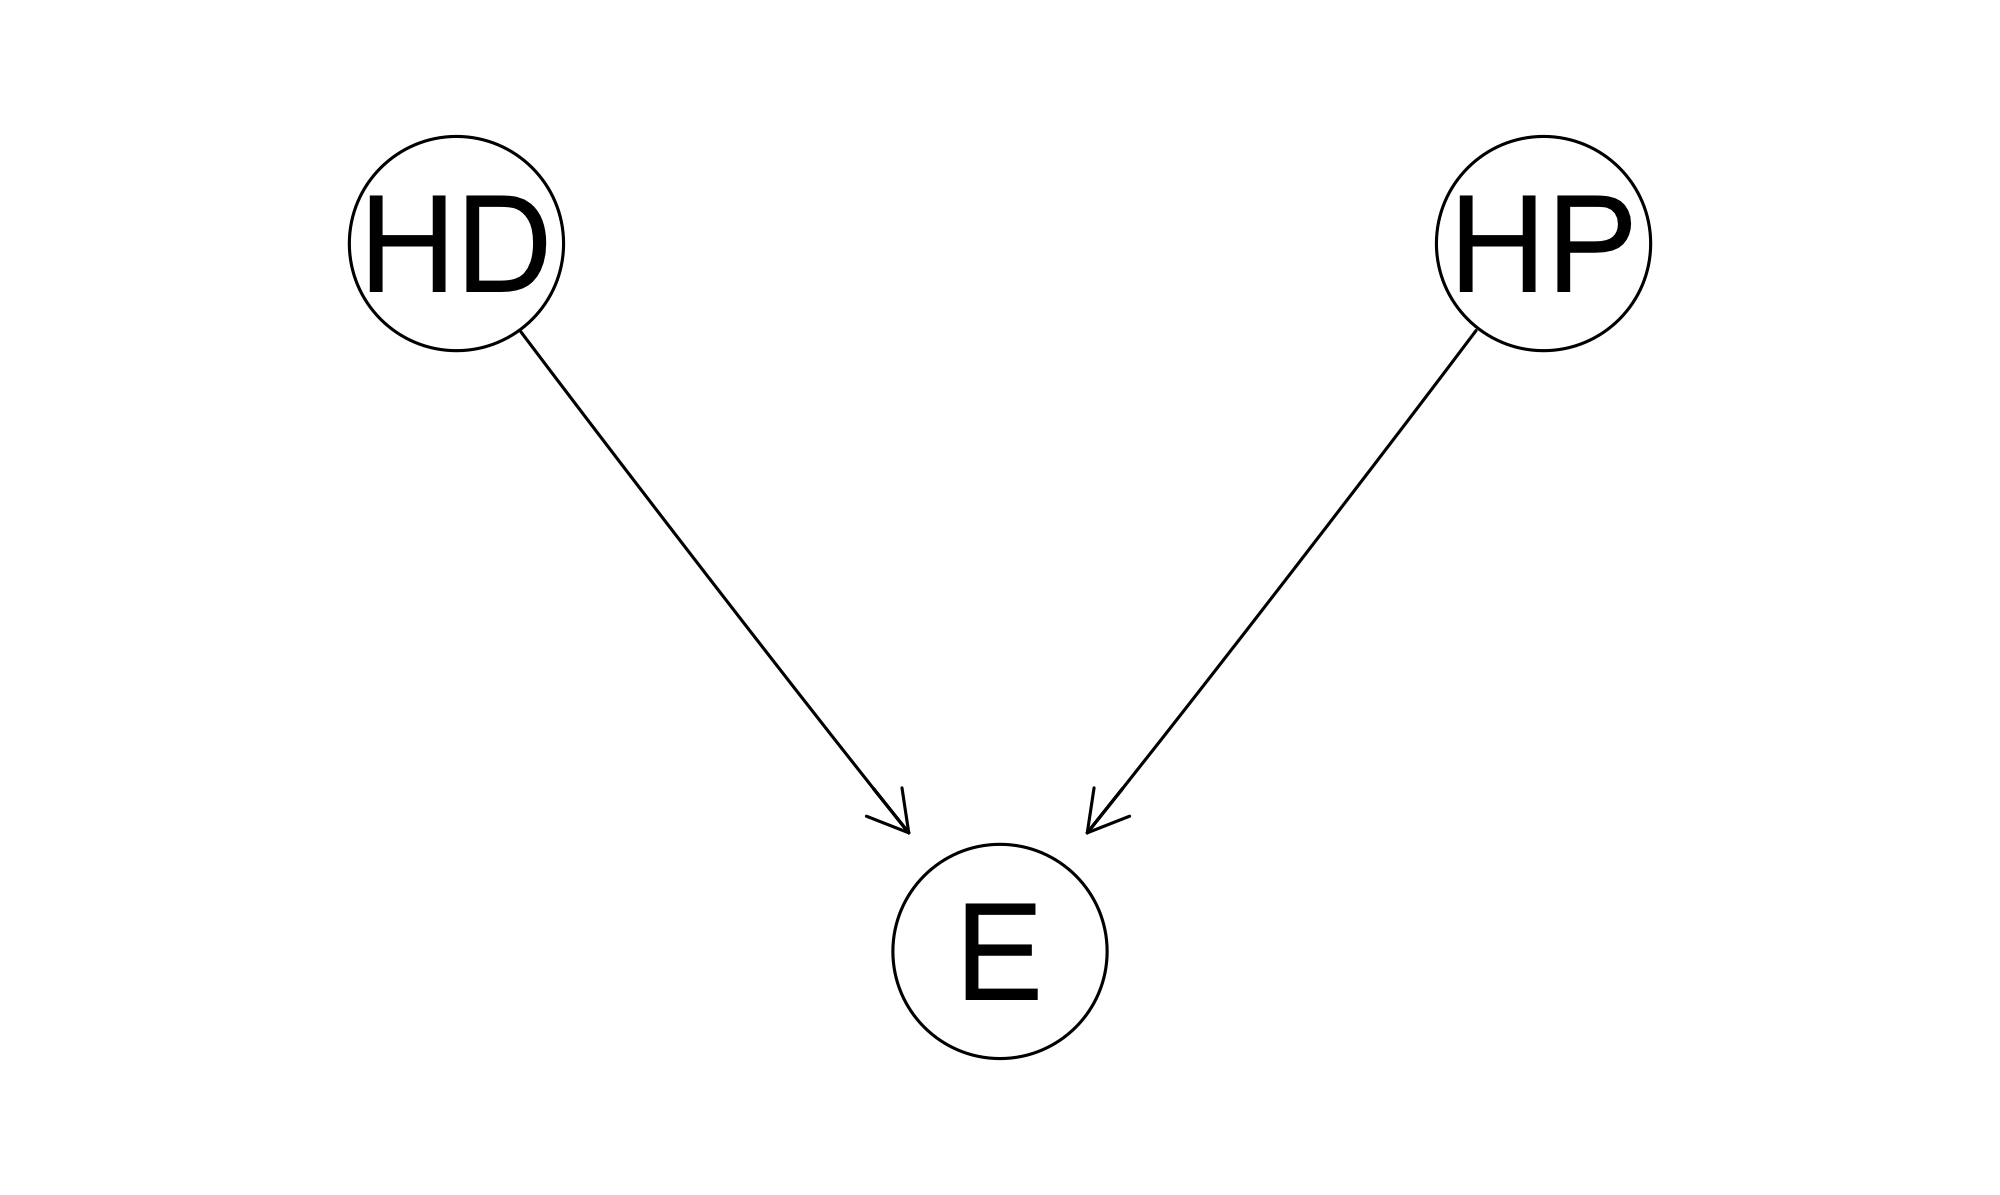
\includegraphics[scale = 0.08]{STMdag.png}}
        {\caption{\footnotesize Graphic model of Small Town Murder}\label{fig:bayes_test4}}
        \ffigbox{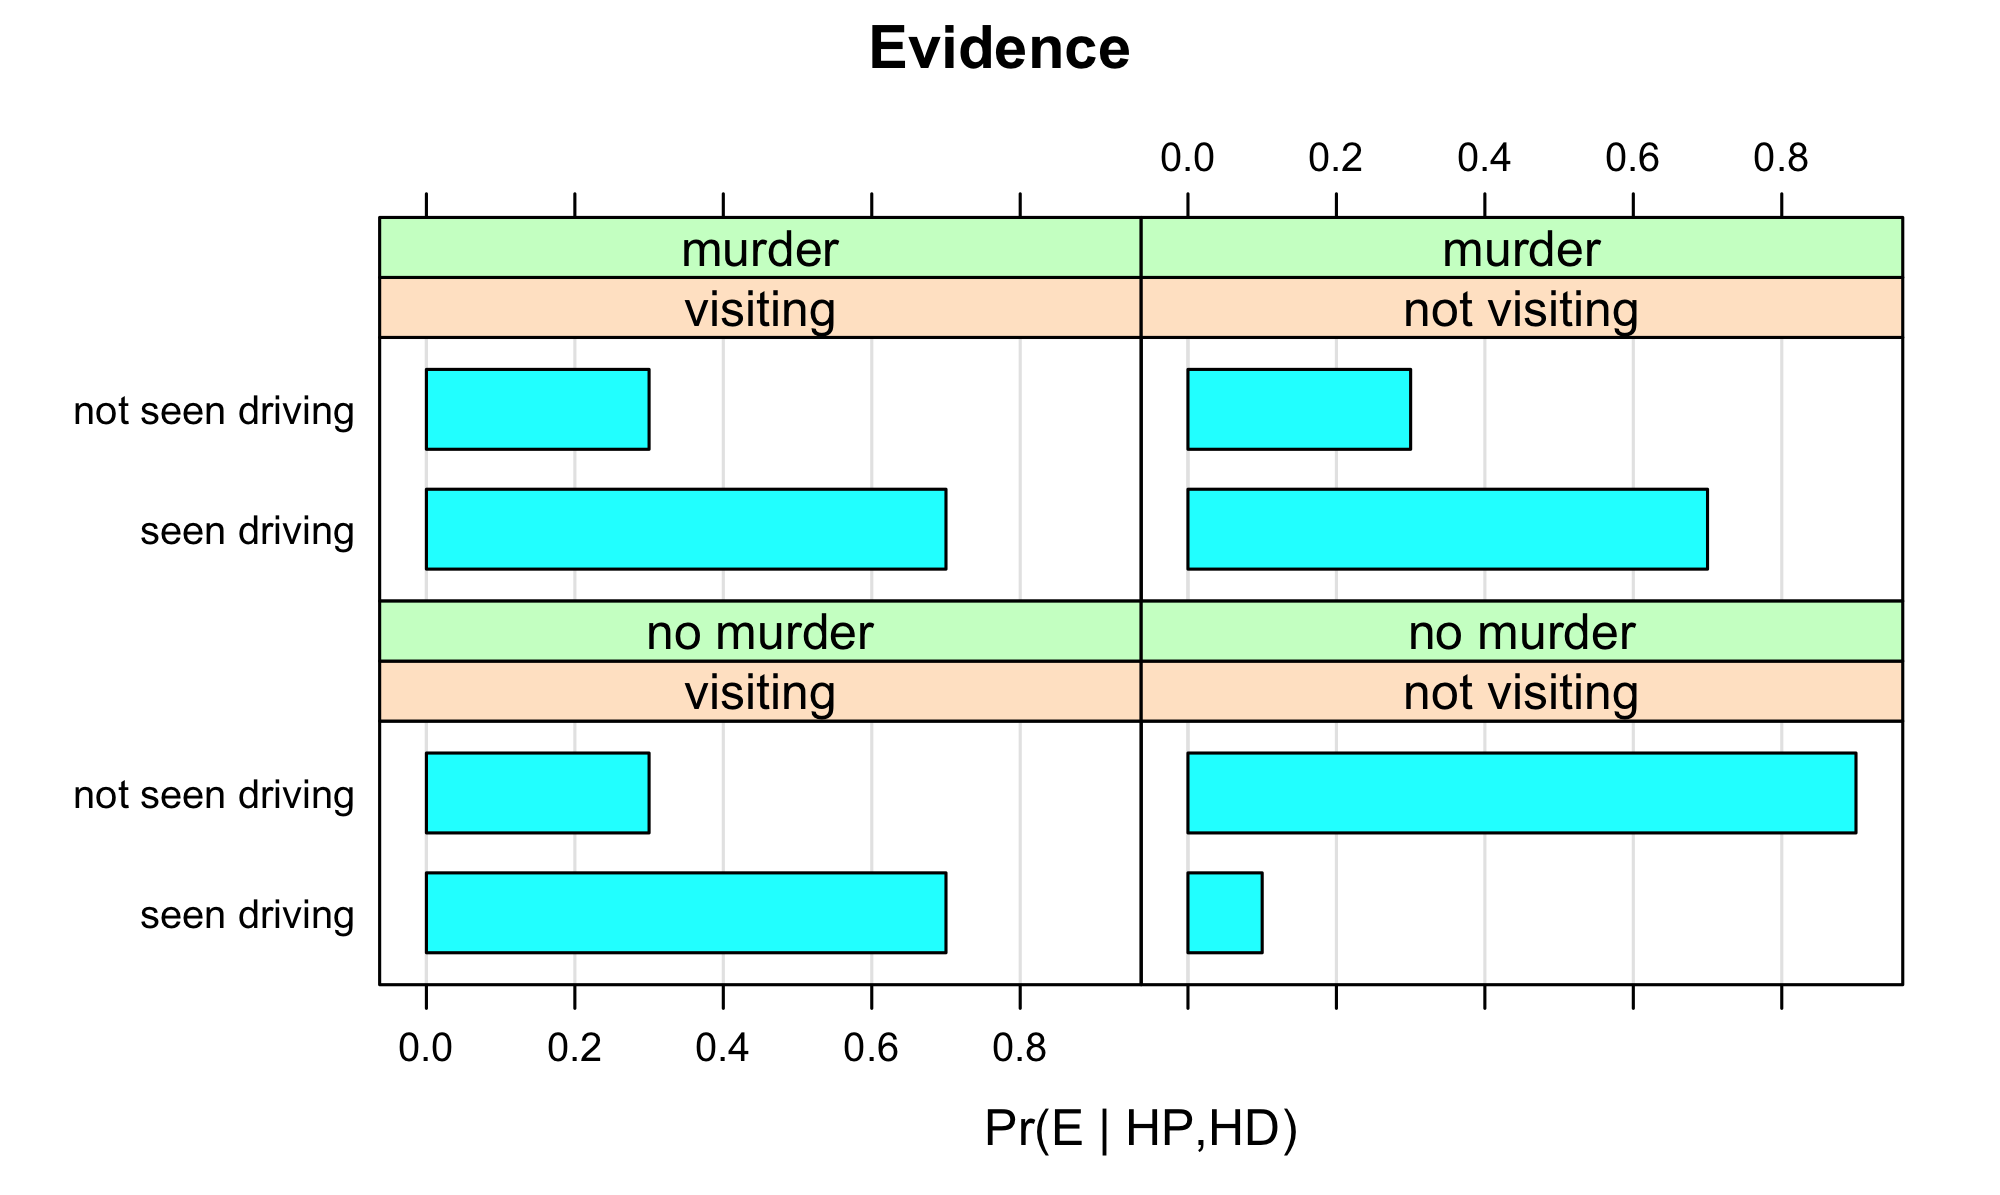
\includegraphics[scale = 0.08]{STMpt.png}}{
            \caption{\footnotesize Probability distribution of $E$}\label{fig:bayes_test6}}
    \end{floatrow}
\end{figure}

\%

\noindent
 Following the calculations in
\citep{dezoete2019ResolvingSocalledProbabilistic}, for exclusive and
exhaustive hypotheses, \(LR(E,H_d,\neg H_d)=1.75\), and similarly,
\(LR(E,H_p, \neg H_p)=1.75\), since \(P(E\vert H_d)=0.7\) and
\(P(E\vert \neg H_d)=0.4\). The likelihood ratio of the evidence, if it
is measured against exclusive and exhaustive hypotheses, is not equal to
one.\footnote{ \cite{dezoete2019ResolvingSocalledProbabilistic} offer a slightly different solution to the problem. They construct a Bayesian network with three hypotheses, also exhaustive and exclusive: in town to visit mother, in town to murder, out of town.}
Such considerations should also generalize to other paradoxes of
relevance.\\
\% \%For instance, in the twins problem, the LR is 1 if the hypotheses
are:
\texttt{the\ suspect\ committed\ the\ crime\textquotesingle{},\ and}the
suspect's twin brother committed the crime', but is not 1 f we consider
the fairly natural hypothesis that the defendant is innocent.
\%Similarly, \%In the food tray example, Bayesian network analysis shows
that the value of the evidence `prisoner withholds tray' for the
question who started the fight depends on a range of uncertain events
and other pieces of evidence (such as whether indeed a parcel he was
supposed to obtain was withheld; whether the prisoner inquired about
this; whether and how this inquiry was answered). Considered in this
context, the piece of evidence will not have a likelihood ratio of one
with respect to at least some choice of sensible hypotheses. \%

The general problem with the paradoxes of relevance is that in complex
situations there is no single likelihood ratio that corresponds to a
single piece of evidence. The problematic scenarios focus on a single
likelihood ratio based on non-exclusive or non-exhaustive hypotheses.
However, evidence can be relevant so long as it has a probabilistic
impact on a sub-hypothesis involved in the case, even without having a
recognizable probabilistic impact on the prosecutor's or defense's
ultimate hypotheses. When this happens, it is relevant, in agreement
with Rule 401 of the Federal Rules of Evidence. Bayesian networks help
to see how pieces of evidence can increase or decrease the probability
of different sub-hypotheses
\cite{dezoete2019ResolvingSocalledProbabilistic}.

\%recommend relying on a Bayesian network to investigate in an orderly
manner the way in which pieces of evidence and hypotheses
interact.\todo{no one said the interact in an orderly manner. ;) } \%in
an orderly manner.

\section*{References}\label{references}
\addcontentsline{toc}{section}{References}

\hypertarget{refs}{}
\hypertarget{ref-aitken2010fundamentals}{}
Aitken, C., Roberts, P., \& Jackson, G. (2010). Fundamentals of
probability and statistical evidence in criminal proceedings
(Practitioner Guide No. 1), Guidance for judges, lawyers, forensic
scientists and expert witnesses. \emph{Royal Statistical Society's
Working Group on Statistics and the Law}.

\hypertarget{ref-donnelly1999DNADatabaseSearches}{}
Donnelly, P., \& Friedman, R. D. (1999). DNA Database Searches and the
Legal Consumption of Scientific Evidence. \emph{Michigan Law Review},
\emph{97}(4), 931.

\hypertarget{ref-enfs2015}{}
ENFSI. (2015). \emph{Guidelines for evaluative reporting in forensic
sciences}.

\hypertarget{ref-NRCI1992}{}
National Research Council. (1992). \emph{DNA technology in forensic
science \textup{{[}NRC I{]}}}. Committee on DNA technology in Forensic
Science, National Research Council.

\hypertarget{ref-NRCII1996}{}
National Research Council. (1996). \emph{The evaluation of forensic DNA
evidence \textup{{[}NRC II{]}}}. Committee on DNA technology in Forensic
Science, National Research Council.

\hypertarget{ref-robertson2016interpreting}{}
Robertson, B., Vignaux, G., \& Berger, C. (2016). \emph{Interpreting
evidence: Evaluating forensic science in the courtroom}. John Wiley \&
Sons.

\hypertarget{ref-Royall1997}{}
Royall, R. M. (1997). \emph{Statistical evidence: A likelihood
paradigm}. Chapman; Hall/CRC.

\hypertarget{ref-triggsCommentWhyEffecta}{}
Triggs, C. M., \& Buckleton, J. S. (2004). Comment on: Why the effect of
prior odds should accompany the likelihood ratio when reporting DNA
evidence. \emph{Law, Probability and Risk}, \emph{3}, 73--82.

\end{document}
